% !TEX TS-program = pdflatex
% !TEX encoding = UTF-8 Unicode
% !TEX root = ./paper.tex

% This is a simple template for a LaTeX document using the "article" class.
% See "book", "report", "letter" for other types of document.

\documentclass[12pt]{article} % use larger type; default would be 10pt

% Fonts
\usepackage{times}

\usepackage{setspace}
	\doublespacing

\usepackage{textcomp}

\usepackage{textcase}
\usepackage{xcolor}


\usepackage[utf8]{inputenc} % set input encoding (not needed with XeLaTeX)

%%%%%%%%%
% Page
%%%%%%%%%

\usepackage{geometry} % to change the page dimensions
	\geometry{letterpaper} % or a4paper or letterpaper (US) or a5paper or....
	\geometry{margin=1in} % for example, change the margins to 2 inches all round
	% \geometry{landscape} % set up the page for landscape

\usepackage{graphicx} % support the \includegraphics command and options
% \usepackage[parfill]{parskip} % Activate to begin paragraphs with an empty line rather than an indent

%%% PACKAGES
\usepackage{booktabs} % for much better looking tables
\usepackage{array} % for better arrays (eg matrices) in maths

\usepackage{paralist} % very flexible & customisable lists (eg. enumerate/itemize, etc.)
\usepackage{enumitem} % Remove spacing
\setlist{nolistsep}   %     between list items

\usepackage{verbatim} % adds environment for commenting out blocks of text & for better verbatim
\usepackage{subfig} % make it possible to include more than one captioned figure/table in a single float
% These packages are all incorporated in the memoir class to one degree or another...

%%% HEADERS & FOOTERS
\usepackage{fancyhdr} % This should be set AFTER setting up the page geometry
	\pagestyle{fancy} % options: empty , plain , fancy
	\renewcommand{\headrulewidth}{0pt} % customise the layout...
	\lhead{}\chead{}\rhead{}
	\lfoot{}\cfoot{\thepage}\rfoot{}


%%% SECTION TITLE APPEARANCE
%\usepackage{sectsty}
	% \allsectionsfont{\normalfont\Large\bfseries\singlespacing} % (See the fntguide.pdf for font help) \mdseries
	% (This matches ConTeXt defaults)

\usepackage{titlesec}
	\titleformat{\chapter}[display] %[display] puts the title chapter on a separate line
		{\normalfont\huge\bfseries}{\chaptertitlename\ \thechapter}{20pt}{\Huge}
	\titleformat{\section}
		{\singlespacing\normalfont\Large\bfseries}{\thesection}{1em}{\vspace{-2ex}}
	\titleformat{\subsection}
		{\singlespacing\normalfont\large\bfseries}{\thesubsection}{1em}{\vspace{-2ex}}
	\titleformat{\subsubsection}
		{\singlespacing\normalfont\normalsize\bfseries}{\thesubsubsection}{1em}{\vspace{-2ex}}

% paragraph
%\setlength{\parskip}{1cm plus4mm minus3mm}
\setlength{\parindent}{0.5cm}

\titlespacing{\paragraph}{%
  0pt}{%              left margin
  0.5\baselineskip}{% space before (vertical)
  0.5em}%               space after (horizontal)

\usepackage{titling}
	\setlength{\droptitle}{-6em}
	\posttitle{\par\end{center}\vspace{-4em}\vskip 1em\singlespacing\normalfont}

%	\titleformat*{\section}{\fontsize{16}{18}\bfseries\textrm\textsc}
%	\titleformat*{\subsection}{\fontsize{14}{16}\bfseries\textrm}
%	\titleformat*{\subsubsection}{\fontsize{12}{14}\bfseries\textrm}



%%% ToC (table of contents) APPEARANCE
\usepackage[nottoc,notlof,notlot]{tocbibind} % Put the bibliography in the ToC
\usepackage[titles,subfigure]{tocloft} % Alter the style of the Table of Contents
	\renewcommand{\cftsecfont}{\rmfamily\mdseries\upshape}
	\renewcommand{\cftsecpagefont}{\rmfamily\mdseries\upshape} % No bold!

% Drafting
\usepackage{draftcopy}
%	\lhead{\huge  \color{black!13} {DRAFT | DRAFT | DRAFT | DRAFT} }
%	\lfoot{\huge  \color{black!13} {DRAFT | DRAFT | DRAFT | DRAFT} }

% Comments
\usepackage{comment}

% images
\DeclareGraphicsExtensions{.pdf,.png,.jpg}
\usepackage{wrapfig}
\usepackage{float}

% Bibliography
\usepackage[font={small,it}]{caption}
\usepackage[sort&compress,comma,square,super]{natbib}         	% bibliography style

%\usepackage[colorlinks]{hyperref}    	% better urls in bibliography
\usepackage{hyperref}

\renewcommand{\refname}{\vspace{-3ex}}	% no title
\bibliographystyle{IEEEtranN}			% standard formatting, ieee
%\bibliographystyle{plainnat}			% standard formatting, ieee

%%%	Paper Guidelines
%%%		Be written in English.
%%%		Adhere to an 18-page limit. This limit includes the introduction, text, tables, data, illustrations, and appendices. References are not included in the 18-page limit.
%%%		Be submitted on 8-1/2 X 11 inch single-sided sheet1s of paper, double-spaced, with page numbers at the bottom.
%%%		Have page margins of at least 1 inch.
%%%		Use 12 point or larger Arial or Times New Roman font for the body of the report.
%%%		Captions accompanying pictures and graphs, as well as citations for references, may be single-spaced and in a smaller point size.

\newcommand{ \titleText } {Post-Disaster Recovery by Rapid High Resolution Aerial Imaging and Indoor 3D Mapping with Autonomous Quadrotor UAVs driven by Computer Vision Feature Targeting and Real-time Victim Recognition}

\title{ \titleText }
\chead{\footnotesize \normalfont \parbox{16cm} {\centering{\textbf{\textsc{ \textrm{ \titleText } }}}} }

% \author{Paras Jain and Ajay Jain, Monta Vista High School}
% \date{October 3rd, 2013} % Activate to display a given date or no date (if empty),


\author{\vspace{0ex}}
\date{\vspace{-13ex}}


\begin{document}
\begin{onehalfspacing}
	\maketitle
\end{onehalfspacing}

% !TEX root = ../paper.tex

\section{Introduction}						% 2-3 pages

%%%	Introduction: the "why" section (2-3 pages)
%%%	*	Start with a broad picture of the problem you have chosen to study and why it is interesting.
%%%	*	Provide a brief review of pertinent scientific literature, describe what information is missing and how your work addresses this gap in the literature.
%%%	*	Previous relevant publications and patents must be properly cited in the text of the Research Report and included in the Reference section of your report.
%%%	*	Describe the specific problem to be solved, the research question to be answered, the hypothesis(es) to be tested, or the product to be developed (if any).
%%%	*	Provide a brief rationale for the research, and why the work is important.







% Brief
% Try to put a lot of citations here since it is a brief
\textbf{Using our sub-\$500 unmanned aerial vehicles (UAVs), we can save thousands of victims of floods, earthquakes, hurricanes and other disasters with faster and more effective response.} We created a hardware and software platform to produce aerial maps for first responders. 3D indoor models are sent to remote doctors for victim diagnosis. Victims are automatically detected so rescuers can be quickly dispatched to people in need.

\begin{figure}[H]
	\begin{minipage}{.5\textwidth}
		\caption{Flying quadrotor UAV \cite{Wiki:ARDrone}}
		\centering
			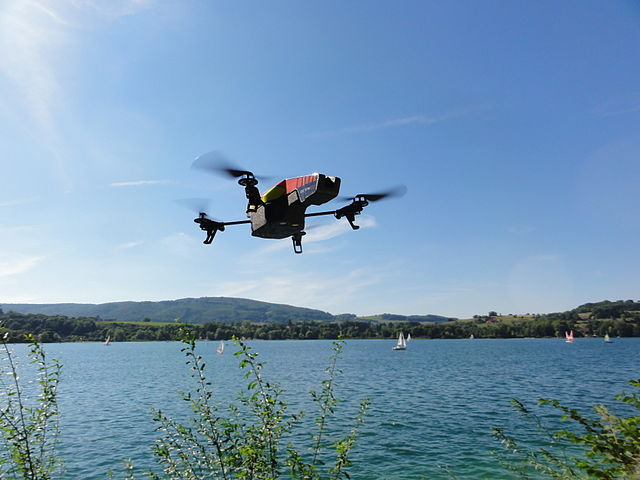
\includegraphics[width=0.95\linewidth]{illustrations/ardrone}
	\end{minipage}
	\begin{minipage}{.5\textwidth}
		\caption{Mounted phone imaging unit}
		\centering
			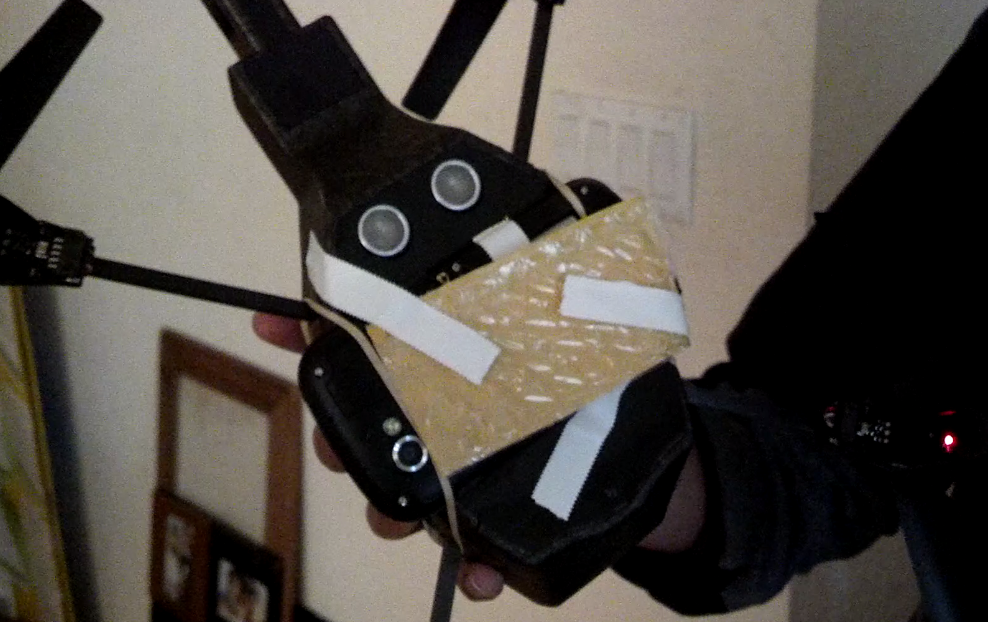
\includegraphics[width=0.95\linewidth]{illustrations/mounted}
	\end{minipage}
\end{figure}

\subsection{Brief}


\subsubsection{Project Components} % what else should this be?
\begin{description}
	\item[Autonomous Quadrotor UAV for Aerial Imaging] progressively captures up to $5 cm$ resolution aerial imagery suitable for facial recognition for under $\$500$
	\item[Agile Quadrotor for Indoor 3D Mapping] maps the interiors of buildings too dangerous to enter with a consumer level 3D camera
	\item[Central Image Processing Server] that all drones communicate with. \textit{Stitches images}, \textit{assembles 3D point clouds}, and \textit{controls the drone network}
	\item[Rapid multi-pass facial recognition] can process gigabytes of high resolution imagery to locate victims performantly
\end{description}


% Brief Aerial Mapping
\subsubsection{Problem: Aerial Mapping}
\noindent
During Hurricane Sandy and the Boston bombings, first responders used commercial level aerial imagery to coordinate search and rescue efforts. \cite{Martinez:BostonBombingAerialImagery} Aerial imagery is \textbf{critical to disaster response---responders can prioritize recovery efforts with increased situational awareness}. High resolution aerial imagery thereby maximizes rescue resources and helps to \textbf{save more lives}. By far, the most commonly used tool currently is Google Earth, however with extremely low resolutions ranging from 1m to 15m making \textit{\textbf{current imagery inadequate}}. \cite{Google:GoogleEarthSpec}

\noindent
Even with high resolution maps, responders need immediate, up-to-date maps to locate damaged areas; this requirement makes any mapping technology that is not real-time or rapidly deployable inapplicable. % chose a different word for inapplicable as satellite is still useful, it just does not solve the problem at hand
% The only applicable technology left is the use of aircraft to survey the area; however, this is expensive, requires trained operator and only offers limited awareness making it difficult to collaborate.
With current imagery and mapping technology, \textbf{automated search for survivors is infeasible}.


% Brief Indoor Searches
\subsubsection{Problem: Indoor Victim Search and Rescue}
\noindent
\textbf{First responders risk their lives} when entering buildings to search for victims. In situations where the disaster involves hazardous agents, like the Fukushima Nuclear Disaster, \textbf{searching for victims may not be possible} given the risk to responders. % cite needed

%Significant prior work has been completed on facial recognition and is very accurate with Haar cascades. % cite needed
%However, such algorithms like the Viola Jones algorithm are relatively slow and are impractical on embedded hardware such as the ARM platform, used to power the imaging UAV in this project.

\subsubsection{Potential Application: Fully Integrated Automated Victim Search in a Disaster}
\noindent
With the high resolution aerial imaging platform developed in this project, \textbf{automatic search for victims has been created, freeing disaster responders to rescue identified targets while removing the need to search indoors. Preliminary results can be available within 15 minutes, upon which a UAV autonomously deploys, images a target and returns}. 




%\subsection{Problem and Potential Applications}
%Aerial searches were used to find the Boston Marathon bomber - however, this effort required many trained police or military pilots to fly specially equipped helicopters in parallel. %CITE	

%This project created a novel system of intelligent drones that act as a group to map and analyze entire cities in real-time. Using a multi-pass approach, we generate imagery that is up to \textbf{an order of magnitude higher resolution than the best available satellite maps}. Each individual drone costs under \$500.

%We created a facial recognition algorithm designed to detect faces quickly in very large images and panoramas. Our system of drones automates victim search and can greatly improve the disaster response process.

%After mapping out a city, drones semi-autonomously generate 3D maps of the interiors of buildings, \textbf{enabling remote diagnosis of victims without endangering first responders}.


\subsection{Motivation - Potential Utility for Rapid Drone based Imagery}
Fresh aerial imagery allows first responders to target highly damaged areas quickly and prioritize rescue efforts. By shifting the time first responders spend searching for victims to rescuing them, more lives can be saved, especially with time critical injuries such as blood loss.

%We created a hardware and software platform to produce aerial maps for first responders.
%Images taken by a high-altitude drone and smartphone are analyzed to identify interest areas and low-altitude drones procure high-resolution imagery.


\subsection{Alternate Solutions}
Unmanned Aerial Vehicles (UAVs) have occasionally been used in search and rescue efforts. However, current imaging approaches have many limitations. Existing models like the Mikrokopter and Aeryon Scout (\autoref{fig:AeryonPhoto}) require direct human control, and video captured needs to be analyzed by operators. Further, these solutions are cost prohibitive (Aeryon Scout is over \$100,000). \cite{aeryonscout:price}

%\begin{wrapfigure}{R}{0.3\textwidth}
%	\caption{Aeryon Scout Pro, $\$107,500$ \cite{aeryonscout:price,Dkroetsch:AeryonPhoto}}
%	\label{fig:AeryonPhoto}
%	\vspace{-3ex}
%	\begin{center}
%		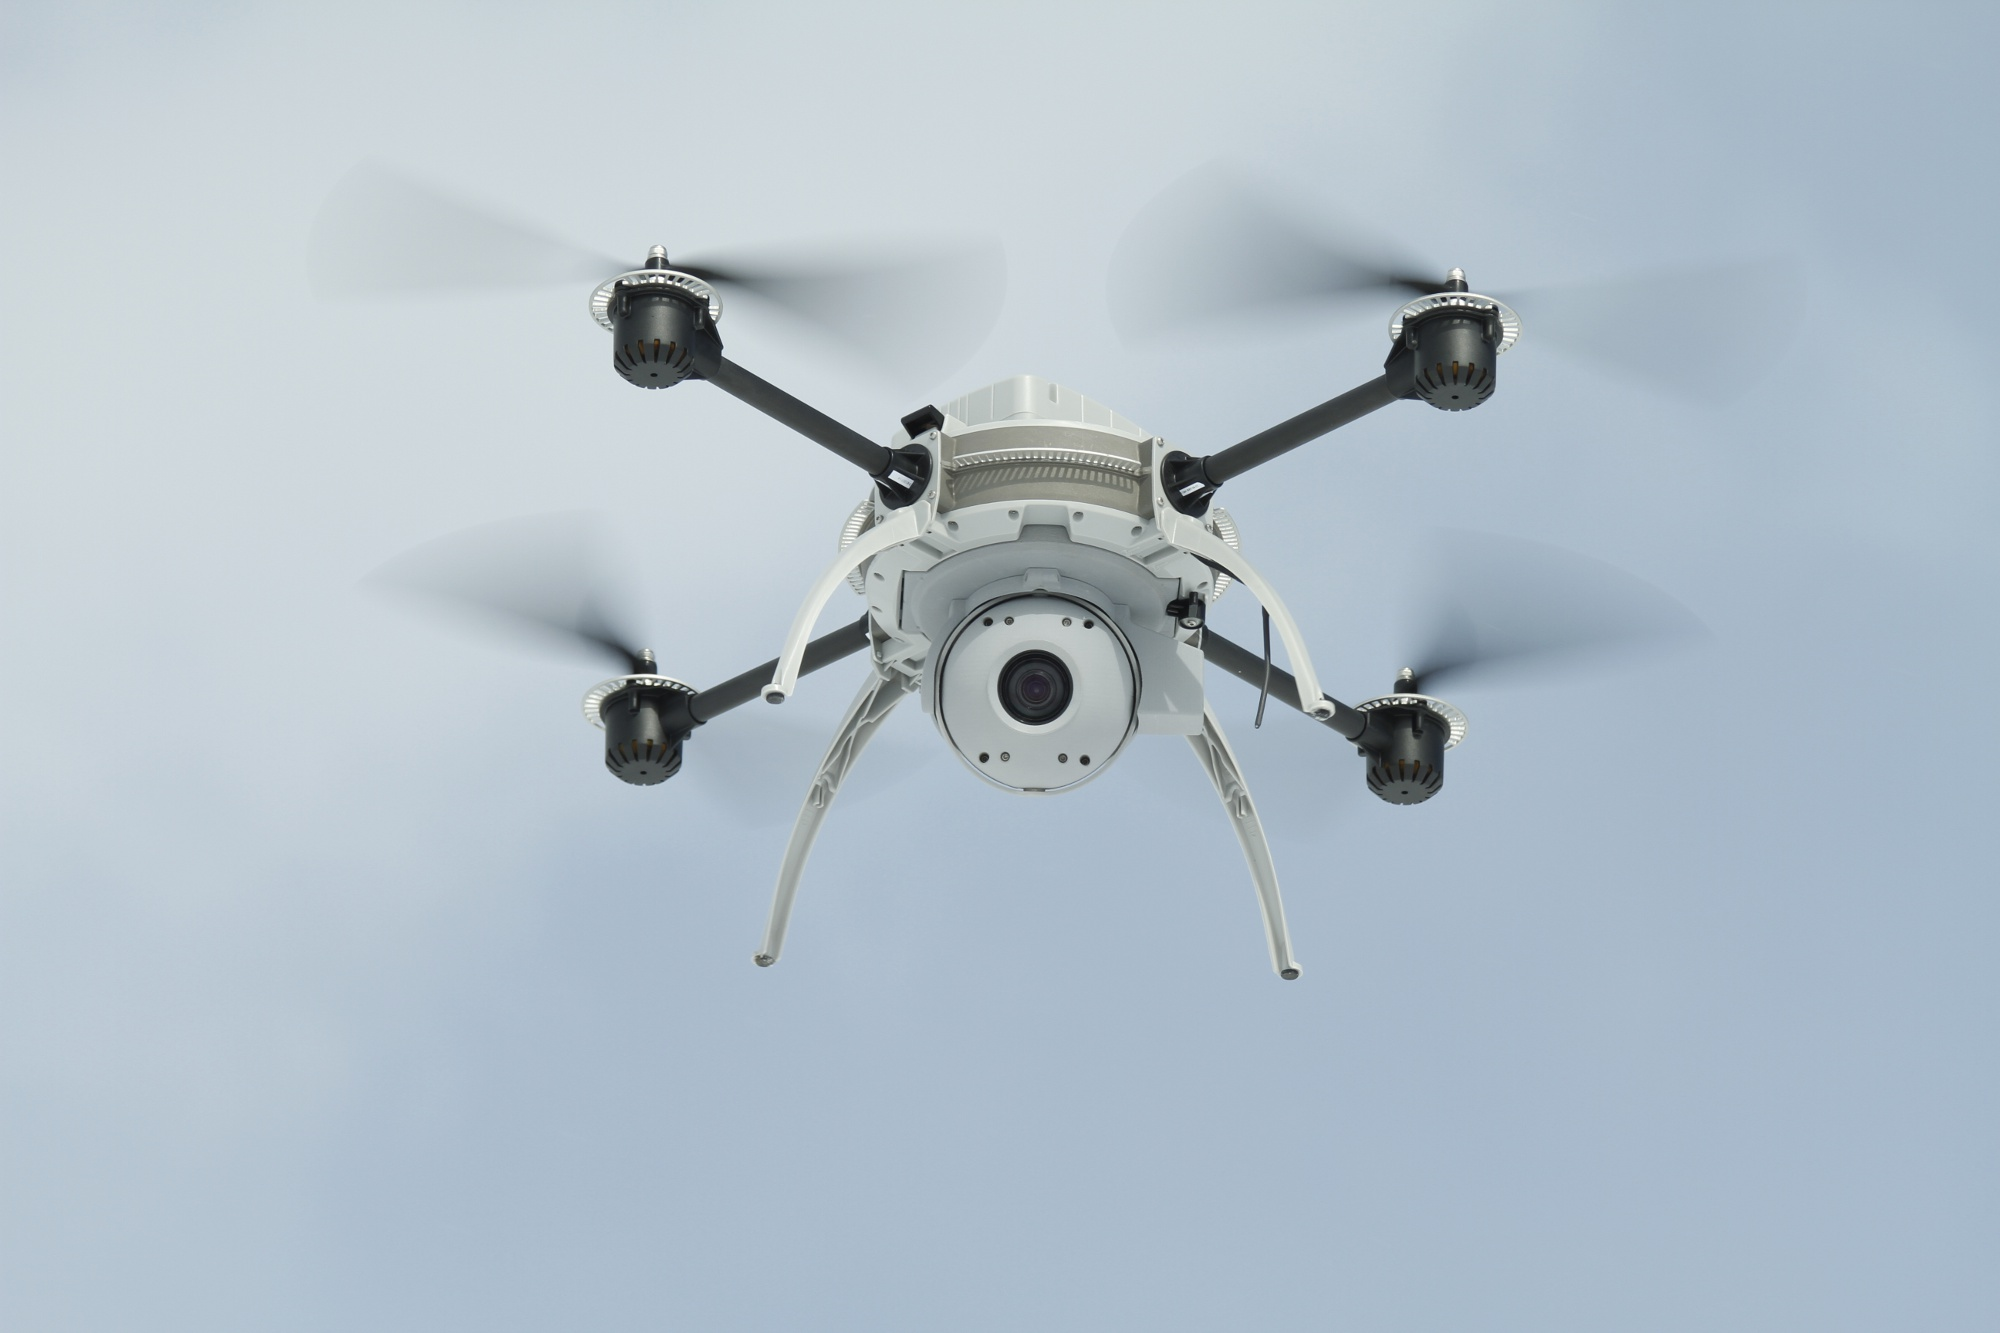
\includegraphics[width=0.29\textwidth]{illustrations/alternate_solutions/uav}
%	\end{center}
%\end{wrapfigure}

Satellites such as GeoEye-I can take 8-10 days to reach the disaster area, post-storm cloud fields can obstruct clear view, and non-military satellite imagery has a capped resolution at $\frac{1}{2}$ meter at best, often at a resolution as low as $15m^2$ per pixel. \cite{Shankland:GeoEyeImagery}

Commercial drones typically range from $\$10,000$ to over $\$100,000$ while providing little additional value for rescue teams as most lack autonomous capabilities, requiring a specially trained operator, making such drones cost-prohibitive for many organizations.
\cite{Campoy:CommercialDronesExpensive}

\subsection{Quadrotor Advantages}
\vspace{1ex}
\begin{onehalfspacing}
	\begin{itemize}
		\item Quadrotors are similar to helicopters but have more maneuverability meaning quadrotors can hover in place, extremely important for aerial photography.
		\item Diametrically opposite blades rotate in the same direction, with one set rotating clockwise and one rotating counter-clockwise.
		\item The counter rotation of adjacent blades results in no net torque on the quadrotor.
		\item VTOLs (Vertical Takeoff and Landing): Drones can launch and land in confined spaces on many terrains
		\item Reduced mechanical complexity means safer and lower cost than helicopters
	\end{itemize}
\end{onehalfspacing}

\subsection{Project Goals}
Our engineering goal is the design and construction of an \textit{affordable} autonomous quadrotor based aerial photography system for rapid acquisition of accurate and up-to-date maps to aid disaster response or commercial interests coupled with indoor 3D scanning to allow responders to locate victims in a damaged building.

\subsection{Engineering Design Criteria}
\vspace{1ex}
\begin{onehalfspacing}
	\begin{enumerate}
		\item Function with daytime environments, winds under 20 km/h
		\item Include GPS and other sensors for navigation
		\item Individual unit less than \$500
		\item High resolution front and bottom cameras to ensure quality imagery.
		\item The UAV should have an angular resolution better than 41cm to beat current satellite imaging technology
	\end{enumerate}
\end{onehalfspacing}

\subsection{Team Contributions}
Team Leader primarily focused on the construction of the quadrotor platform as well as the design and architecture of the distributed server cluster. This included the control systems that drove the quadrotor. Team Leader designed the 3D indoor iteration of the quadrotor which utilized a very heavily modified consumer RGB-D 3D sensor.
Team Member created the image processing toolset and built the 3D stitching pipeline to generate point clouds for interiors of buildings.

% !TEX root = ../paper.tex

\section{Materials and Methods}				% 2-5 pages

%%%	Materials & Methods: the "how" section (2-5 pages)
%%%		Describe how you performed your work, giving sufficient detail so that someone trained in the field is able to understand what you did and can replicate it.
%%%		Include the methods you used, written in a format commonly used in publications in your field of study.
%%%		Do not merely restate a protocol or copy blocks of text; instead, use your own words to describe what you did, referencing key papers where appropriate.
%%%		Explain your personal role in the work and the roles played by others in supporting this work.
%%%		Include, for example, acknowledgments to others in the laboratory for running key instrumentation or other protocols.
%%%		You may refer to others who assisted you by title but do not include any specific names in the body of your Research Report.
%%%		Mention common procedures but there is no need to describe them in detail; provide references to where the method is published.
%%%		All modifications of existing methods should be described.

\subsection{High Level Process}
\vspace{1ex}
\begin{onehalfspacing}
	\begin{enumerate}
		\item A master quadrotor drone captures high altitude imagery of an area by automatically navigating between generated GPS waypoints.
		\item Servers identify SIFT keypoints and stitch images together into map overlays.
		\item Slave quadrotor drones are deployed to keypoint clusters and capture high resolution panoramas.
		\item Indoor 3D maps are generated with drone mounted RGBD cameras.
	\end{enumerate}
\end{onehalfspacing}

\subsection{AR.Drone}

We modified the $\$300$ Parrot AR.Drone 2.0 recreational quadrotor to serve as a base payload carrying platform. The lightweight drone is very inexpensive, although we had to strip much of the protective casing to increase additional cargo capacity. The UAV has a built in frontal camera, with a resolution of $720$p ($1280$×$720$) and a $240$p QVGA high frame rate bottom stabilization camera. The AR.Drone includes a logic board that coordinates the four rotors and stabilizes the craft with sensory input.

Summary of UAV specifications\cite{ardrone2:specs}:
\begin{onehalfspacing}
	\begin{itemize}
		\item Barometer and ultrasonic sensor for altitude measurement
		\item Accelerometer and gyroscope
		\item $1280$×$720$ pixel wide angle front camera
		\item $320$×$240$ pixel QVGA high frame rate bottom camera for measuring ground speed
	\end{itemize}
\end{onehalfspacing}


\textbf{By using off the shelf hardware and modifying it for the project requirements, the price per drone can be kept low due to price savings from large scale mass production}.

\subsubsection{UAV Control}

\begin{onehalfspacing}
	\begin{enumerate}
		\item An operator draws a flight path in Google Earth and way-points are generated. (\autoref{fig:FlightPlan})
		\item The drone is launched and stabilized.
		\item Photos and telemetry collected and transmitted to server.
		\item Flight is adjusted when the drone exits a 3 meter wide corridor between way-points.
		\item The flight plan is sent to the central server to be added as an imaging to the task queue for the drone fleet to deploy a charged UAV.
	\end{enumerate}
\end{onehalfspacing}

\begin{figure}[h!]
	\begin{minipage}{.4\textwidth}
		\caption{Google Earth flight plan}
		\label{fig:FlightPlan}
		\centering 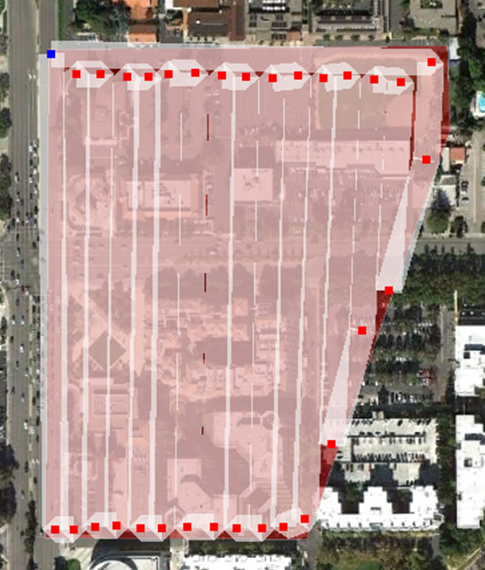
\includegraphics[width=0.9\linewidth]{illustrations/flight_path}
	\end{minipage}%
	\begin{minipage}{.6\textwidth}
		\caption{UAV control flow}
		\label{fig:DroneControl}
		\centering 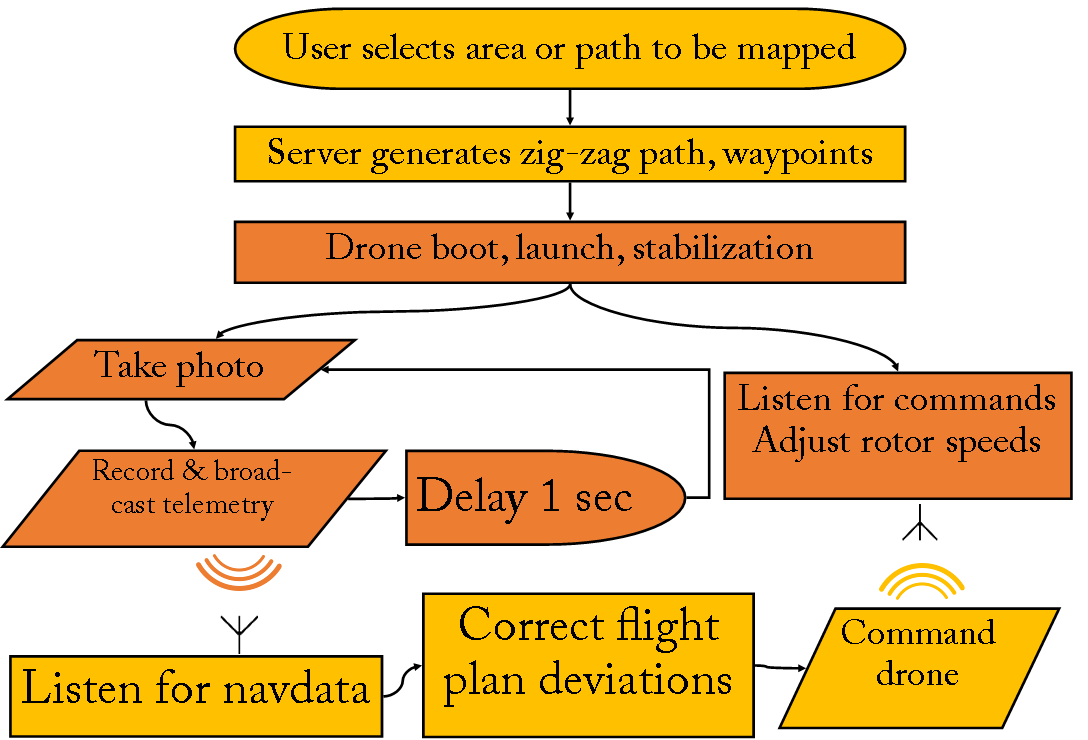
\includegraphics[width=0.9\linewidth]{illustrations/drone_chart}
	\end{minipage}
\end{figure}

\subsection{Central Server}

\begin{figure}[h!]
		\caption{Server Cluster Architecture}
		\label{fig:ServerArch}
		\centering 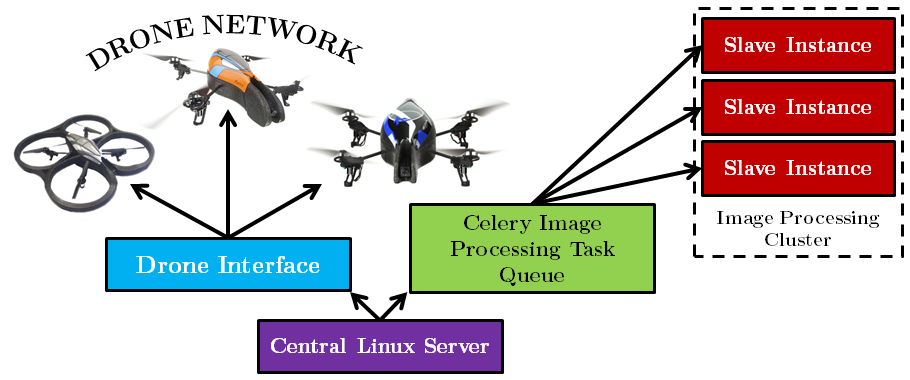
\includegraphics[width=0.9\linewidth]{illustrations/serverarch_lmroman}
\end{figure}

\noindent
A central Linux server acts as a central hub to which every drone connects to. This server handles drone management and acts as a load balancer to the rest of the cluster. As images are collected, it adds tasks to a Celery task queue. Server instances are dynamically created to complete the tasks in the Celery task queue. Such tasks include (but are not limited to) stitching, SIFT keypointing, locating faces and skin tone isolation.

Tasks are completed as a priority queue, allowing image processing jobs that are important (e.g. low resolution keypointing) to be completed first. This distributed system allows the system to become near-infinitely scalable by adding more workers. This process can be automated with a cloud service provider like the Amazon AWS Elastic Compute Cloud where new servers are dynamically provisioned as needed.



\subsection{Phone Telemetry and Ground Imaging}
\textbf{Our final prototype used an inexpensive Android smartphone with a GPS sensor and a 3G data connection to record high resolution imagery and transmit telemetry.} For development, we used the Nexus S, although cheaper and more lightweight devices could easily be substituted. With our \textit{Drone Logger} Android application, an image from the back camera (facing downward when mounted on the UAV) are recorded every second to the phone's internal storage. Depending on the specific device used, different sets of telemetry are available; we captured and transmitted the \textbf{bearing, speed, latitude and longitude}.

% is this the best place to put this? ->
Telemetry is sent to a local or remote server with a public IP address as an HTTP POST request. If telecommunications infrastructure is damaged and a data connection is unavailable on the phone, a portable server and the mounted phone would connect to an adhoc WIFI network.
The AR.Drone creates an In the development of our prototypes, the smartphone, UAV creates a local network with an approximate range of 165 meters.

\subsection{Prototypes}

\subsubsection{V1 $-$ Drone bottom stabilization camera}
Our initial prototype relied on the bottom facing stabilization camera bundled with the AR Drone. Using it for map creation would have minimized the overall costs, but the camera is of too low resolution ($240$p) for workable imagery.

\subsubsection{V2 $-$ Drone Mounted Arduino and Sensors (\autoref{fig:ArduinoDrone})}
To add cameras and additional sensors to the UAV, we mounted an Adruino microcontroller. This gave us the freedom to add additional sensors. However, the asymmetric weight distribution made the drone:
\begin{itemize}
	\item Difficult to isolate issues and to use serial communication
	\item Unstable when mounted
\end{itemize}

\subsubsection{V3 $-$ Android Smartphone and PC Server}
We overcame cost, data transmission and aerodynamic issues in previous prototypes by mounting an Android smartphone on the bottom of the UAV. The phone has several benefit to a custom Adruino based system:
\begin{enumerate}
	\item Even low-end phones contain many built in sensors, including a GPS and 3G antenna.
	\item The back camera is far superior to the built in stabilization camera of the AR.Drone
	\item Electronics are self-contained, reducing drag on the UAV.
	\item We are able to use the Android APIs to interface with sensors.
	\item The data connection allows the phone to relay telemetry data and receive instructions from a remote server.
\end{enumerate}

However, the heavy phone ($129$ grams) decreased the battery life of the UAV and the maximum altitude. To increase the cargo capacity of the AR.Drone, we removed the drone hull and phone casing. We experimented with increasing lift with helium balloons, as a a $30$ cm balloon can lift $14$ grams.

% !TEX root = ../paper.tex

\section{Results}							% 4-5 pages

Our system captures outdoor aerial imagery, First Person View panoramas and 3D indoor point clouds.
Each intelligent quadrotor drone is under $\$500$ per unit. It has a maximum angular resolution of under $5
cm$, while the GeoEye1 satellite has an angular resolution of 41 cm; our drones are almost an order of
magnitude better. \footnote{Resolution in the context of aerial imagery is defined to be the minimum distance between two resolvable features}

\subsection{Map Stitching}

% Brief
% % Indivbidual frames from the quad are deconvoluted, removing blur
% A - process as spec'ed, slow but accurate due to SIFT
% % SIFT keypointing
% % % Corresponding keypoints
% % Overlaying maps
% Commercial Hugin processing pipeline created to use more performant stitching process where possible

Raw frames from each drone streamed from the drones for preliminary processing are overlain on Google Maps without stitching to give responders imagery as quickly as possible.

%TODO FINSIH THOUGHT!!!!
%\noindent
%For complete stitching of high resolution imagery
%\begin{enumerate}
%	\item Raw frames are sharpened to increase detail and the quality of the final stitched map
%	\item 
%\end{enumerate}
%However, this algorithm is extremely slow, a trade-off for its increased resilience.

%\noindent
%For reasonable conditions with limited motion blur, stitching work is processed with the Panotools API. \cite{Dersch:Panotools}

Photos are stitched together into full maps with the computer vision library OpenCV \cite{OpenCV:HomePage}. Features are matched with the Scale-invariant feature transform (SIFT). The process can be slow and imperfect, although optimizations are made using the drone flight plan.

Stitched maps: \autoref{fig:KennedySidewalk}, \autoref{fig:DebrisEarth}, \autoref{fig:Playground}, \autoref{fig:HouseStitch}

\subsection{Panoramic Imaging Spheres}
At clusters of image key points, a drone descends to a low altitude and spins in a complete circle while records footage with the $720$p front camera. Frames from this video are stitched together, creating a $360^{\circ}$ panoramic sphere of an area (\autoref{fig:BackyardPanoStitch}, \autoref{fig:StellingStitch} in Illustrations). \textbf{Objects as small as 5 cm are discernible in this panorama, an order of magnitude better than satellite imagery.}
\begin{figure}[H]
  \caption{Full panorama from a backyard sweep}
  \label{fig:BackyardPanoStitch}
  \centering
    \includegraphics[width=\textwidth]{illustrations/maps/backyard_pano_mag}
\end{figure}

\subsection{Face Detection}
\textbf{BRIEF:} Faces are detected within generated panoramas with a two pass algorithm we designed to manage large images. \textbf{Much of the search process in disaster recovery can be automated with our system.}

Facial features are discernible in the panoramic imaging spheres generated by low altitude drones searching for survivors. In order to eliminate the time consuming search process disaster responders must manually do even with aerial imagery, faces are detected and reported to rescuers. We evaluated three existing implementations of face detection algorithms for accuracy over a set of 39 images: the Haar feature detection in OpenCV, the FindFaces Mathematica function and Chan Vese image binarization.

\begin{figure}[h]
	\begin{minipage}{.33\textwidth}
		\caption{ChanVeseBinarize}
		\centering 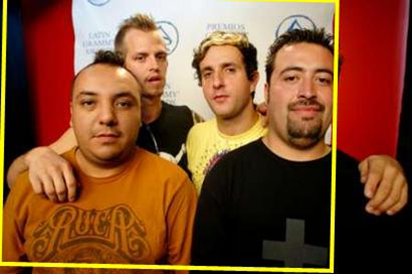
\includegraphics[width=0.95\linewidth]{illustrations/faces/1/ChanVese}
		\centering 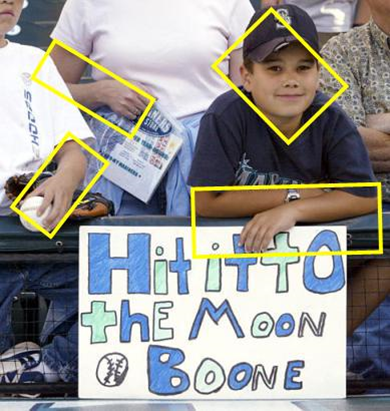
\includegraphics[width=0.95\linewidth]{illustrations/faces/2/ChanVese}
	\end{minipage}
	\begin{minipage}{.33\textwidth}
		\caption{Haar-Feature detection}
		\centering 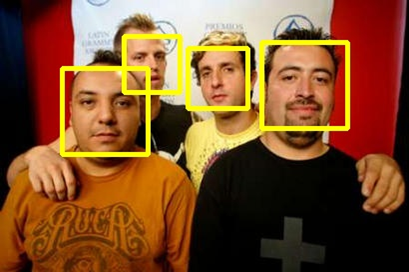
\includegraphics[width=0.95\linewidth]{illustrations/faces/1/Haar}
		\centering 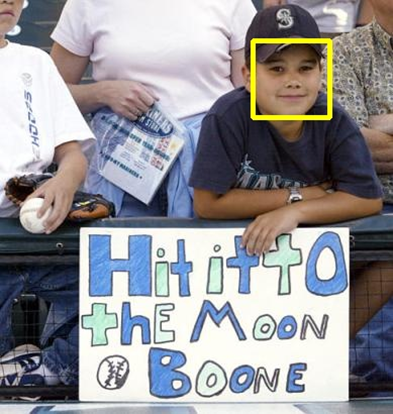
\includegraphics[width=0.95\linewidth]{illustrations/faces/2/Haar}
	\end{minipage}
	\begin{minipage}{.33\textwidth}
		\caption{FindFaces}
		\centering 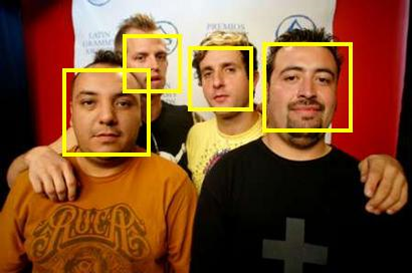
\includegraphics[width=0.95\linewidth]{illustrations/faces/1/FF}
		\centering 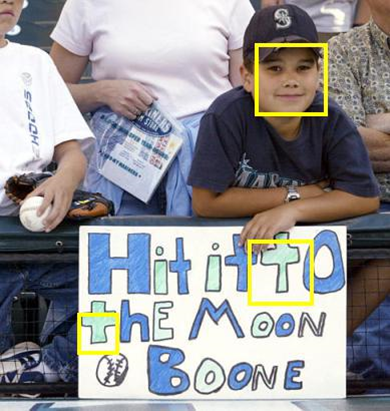
\includegraphics[width=0.95\linewidth]{illustrations/faces/2/FF}
	\end{minipage}
\end{figure}

\begin{figure}[H]
  \caption{Face detection algorithm accuracy comparison}
  \label{fig:FaceDetectionComparison}
  \centering
    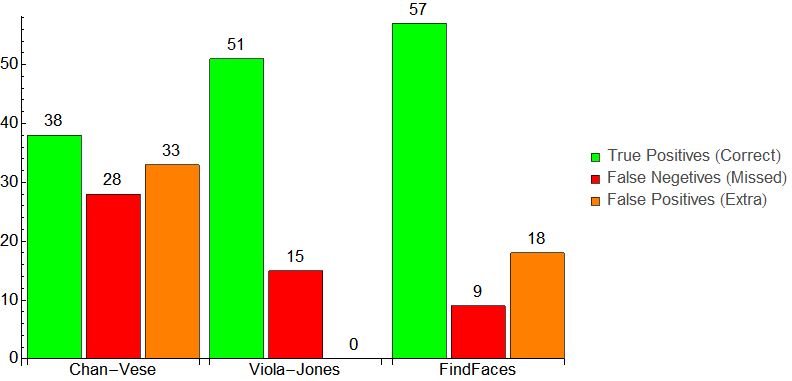
\includegraphics[width=\textwidth]{illustrations/faces/chart}
\end{figure}

\subsubsection{FindFaces and Viola-Jones}

Large XML files are distributed with OpenCV describing pre-generated Haar features. These are created ahead of time with a machine learning algorithm where faces are manually selected in a large data set. The Haar feature detection functions in OpenCV implement the Viola-Jones object detection algorithms. Other features\textemdash trees, eyes, and animals, for example\textemdash can be detected trivially by swapping out the data set.

FindFaces and the Haar feature detection method had few false positives and negatives (extra and missed faces) (\autoref{fig:FaceDetectionComparison}), but perform badly on large images. The image is usually scanned region by region, which is infeasible for our panoramas.

\subsubsection{Chan Vese Image Binarization}

The Chan Vese algorithm segments (splits) an image, locating the boundaries of an image. In the Mathematica ChanVeseBinarize implementation\cite{Wolfram:ChanVese}, objects of a target color are segmented out. By targeting skin tones, specifically orange, we were able to detect exposed skin in an image. Used exclusively for face detection, the algorithm returns many false positives since all skin and orange objects are identified. However, the algorithm can process large images far faster than Haar feature detections and FindFaces. \textbf{To detect faces in large panoramas, we first narrow the possible search space to skin colored areas with ChanVeseBinarize, then apply one of the more robust algorithms to reduce false positives.}

\subsection{3D Point Cloud Generation}

\begin{figure}[h]
	\begin{minipage}{.5\textwidth}
		\caption{Depth map created by RGBD camera.}
		\label{fig:KinectDepth}
		\centering
			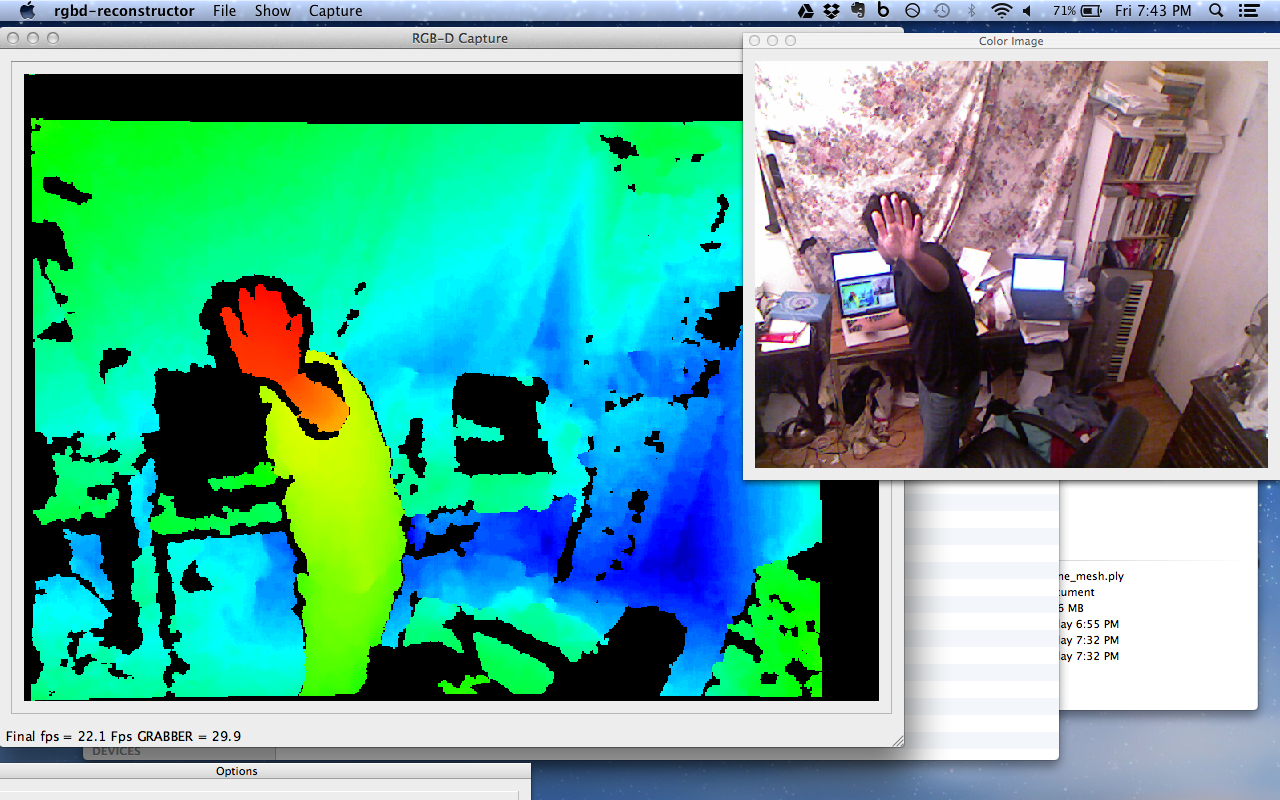
\includegraphics[width=.95\linewidth]{illustrations/clouds/depth}
	\end{minipage}
	\begin{minipage}{.5\textwidth}
		\caption{Generated point cloud. 3D map can be sent to doctors for remote diagnosis of victims.}
		\label{fig:BedPointCloud}
		\centering
			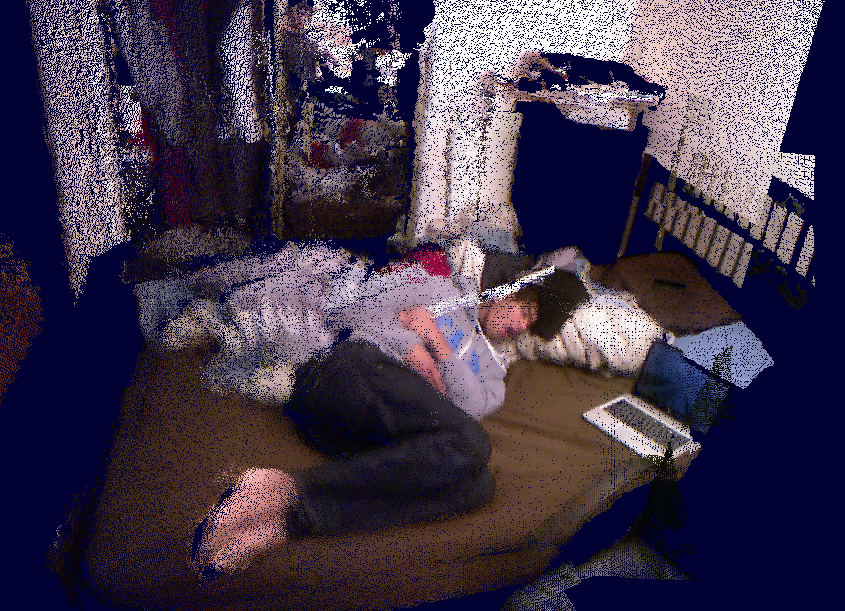
\includegraphics[width=.95\linewidth]{illustrations/clouds/bed}
	\end{minipage}
\end{figure}

Using a stripped down Asus Xtion, a consumer depth camera originally intended for gaming, RGB-D data could be obtained from an drone indoors with limited range (\autoref{fig:KinectDepth}). SLAM (Simultaneous Localization and Mapping) is used to generate 3D point clouds of the interior of a building (\autoref{fig:BedPointCloud}). \textbf{These point clouds can be sent to off-site doctors for remote diagnosis of victims. First responders do not need to enter dangerous collapsing buildings after a disaster until they are certain there is someone in need inside.}

%\begin{figure}[H]
%	\caption{Ground based tether for 3D camera due high bandwidth requirements (400mbps)}
%	\centering
%		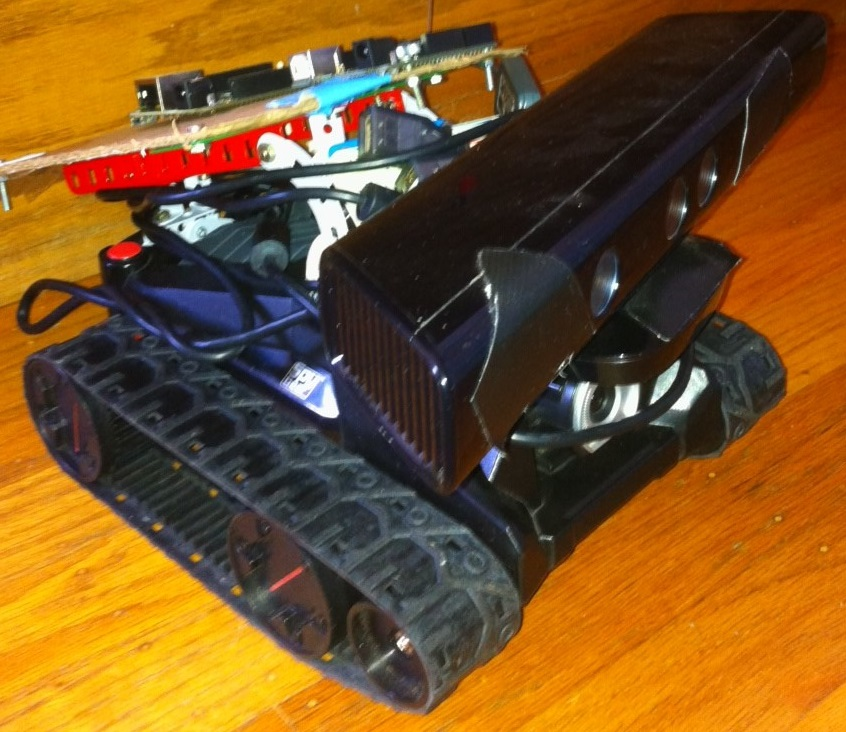
\includegraphics[width=0.5\textwidth]{illustrations/ground}
%\end{figure}

\subsection{Google Earth Map Creation}

Map data with stiches superimposed upon Google Maps is delivered to first responders through KML export for portability and ease of use by First Responders. Pictures are overlaid on a satellite map and oriented and sized from drone telemetry.\footnote{This telemetry includes latitude/longitude, heading, bearing and altitude} \textbf{Operators and first responders can assess damage in regions and determine where help is needed while locating survivors.}

% !TEX root = ../paper.tex
\section{Illustrations}						% 2-4 pages

\begin{figure}[H]
  \caption{Quadrotor dynamics \cite{Kumar:QuadrotorOverview} }
  \centering
    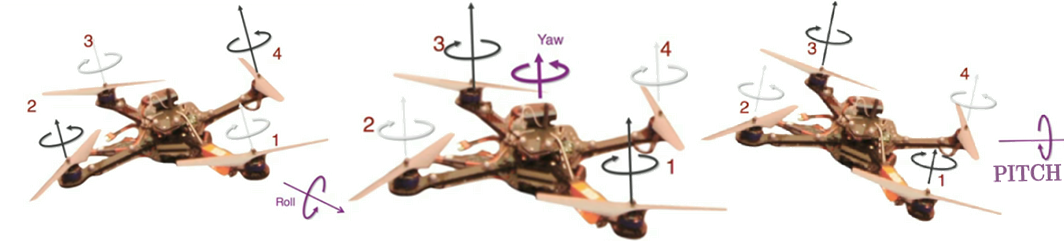
\includegraphics[width=\textwidth]{illustrations/quadcopter_diagram}
\end{figure}

\begin{figure}[h]
	\begin{minipage}{.5\textwidth}
		\caption{Mapping system breakdown}
		\centering
			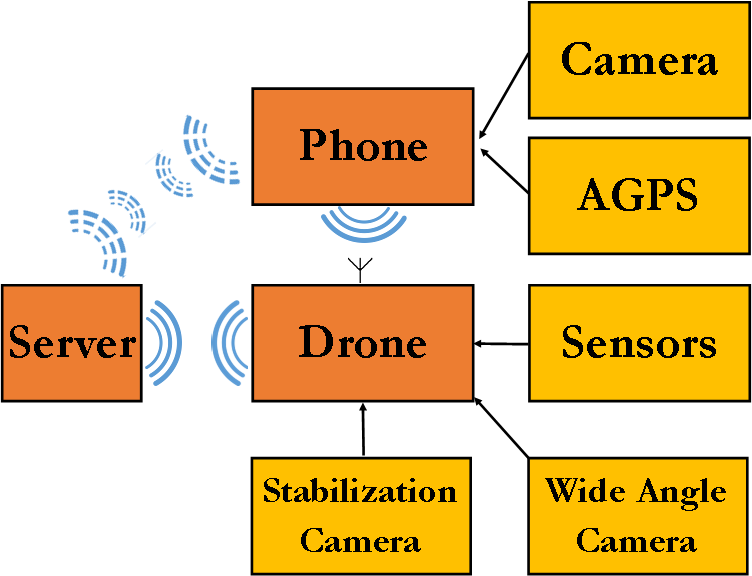
\includegraphics[width=0.95\linewidth]{illustrations/system_chart}
	\end{minipage}
	\begin{minipage}{.5\textwidth}
		\caption{Arduino interfacing with drone}
		\label{fig:ArduinoDrone}
		\centering
			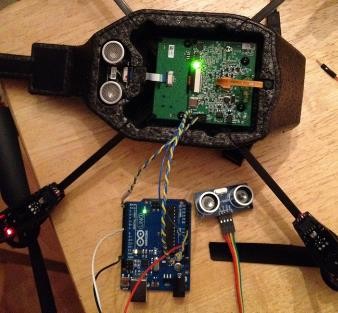
\includegraphics[width=0.95\linewidth]{illustrations/arduino_drone}
	\end{minipage}
\end{figure}

\begin{figure}[h]
	\begin{minipage}{.5\textwidth}
		\caption{Stitch from night-time UAV flyover}
		\label{fig:KennedySidewalk}
		\centering
			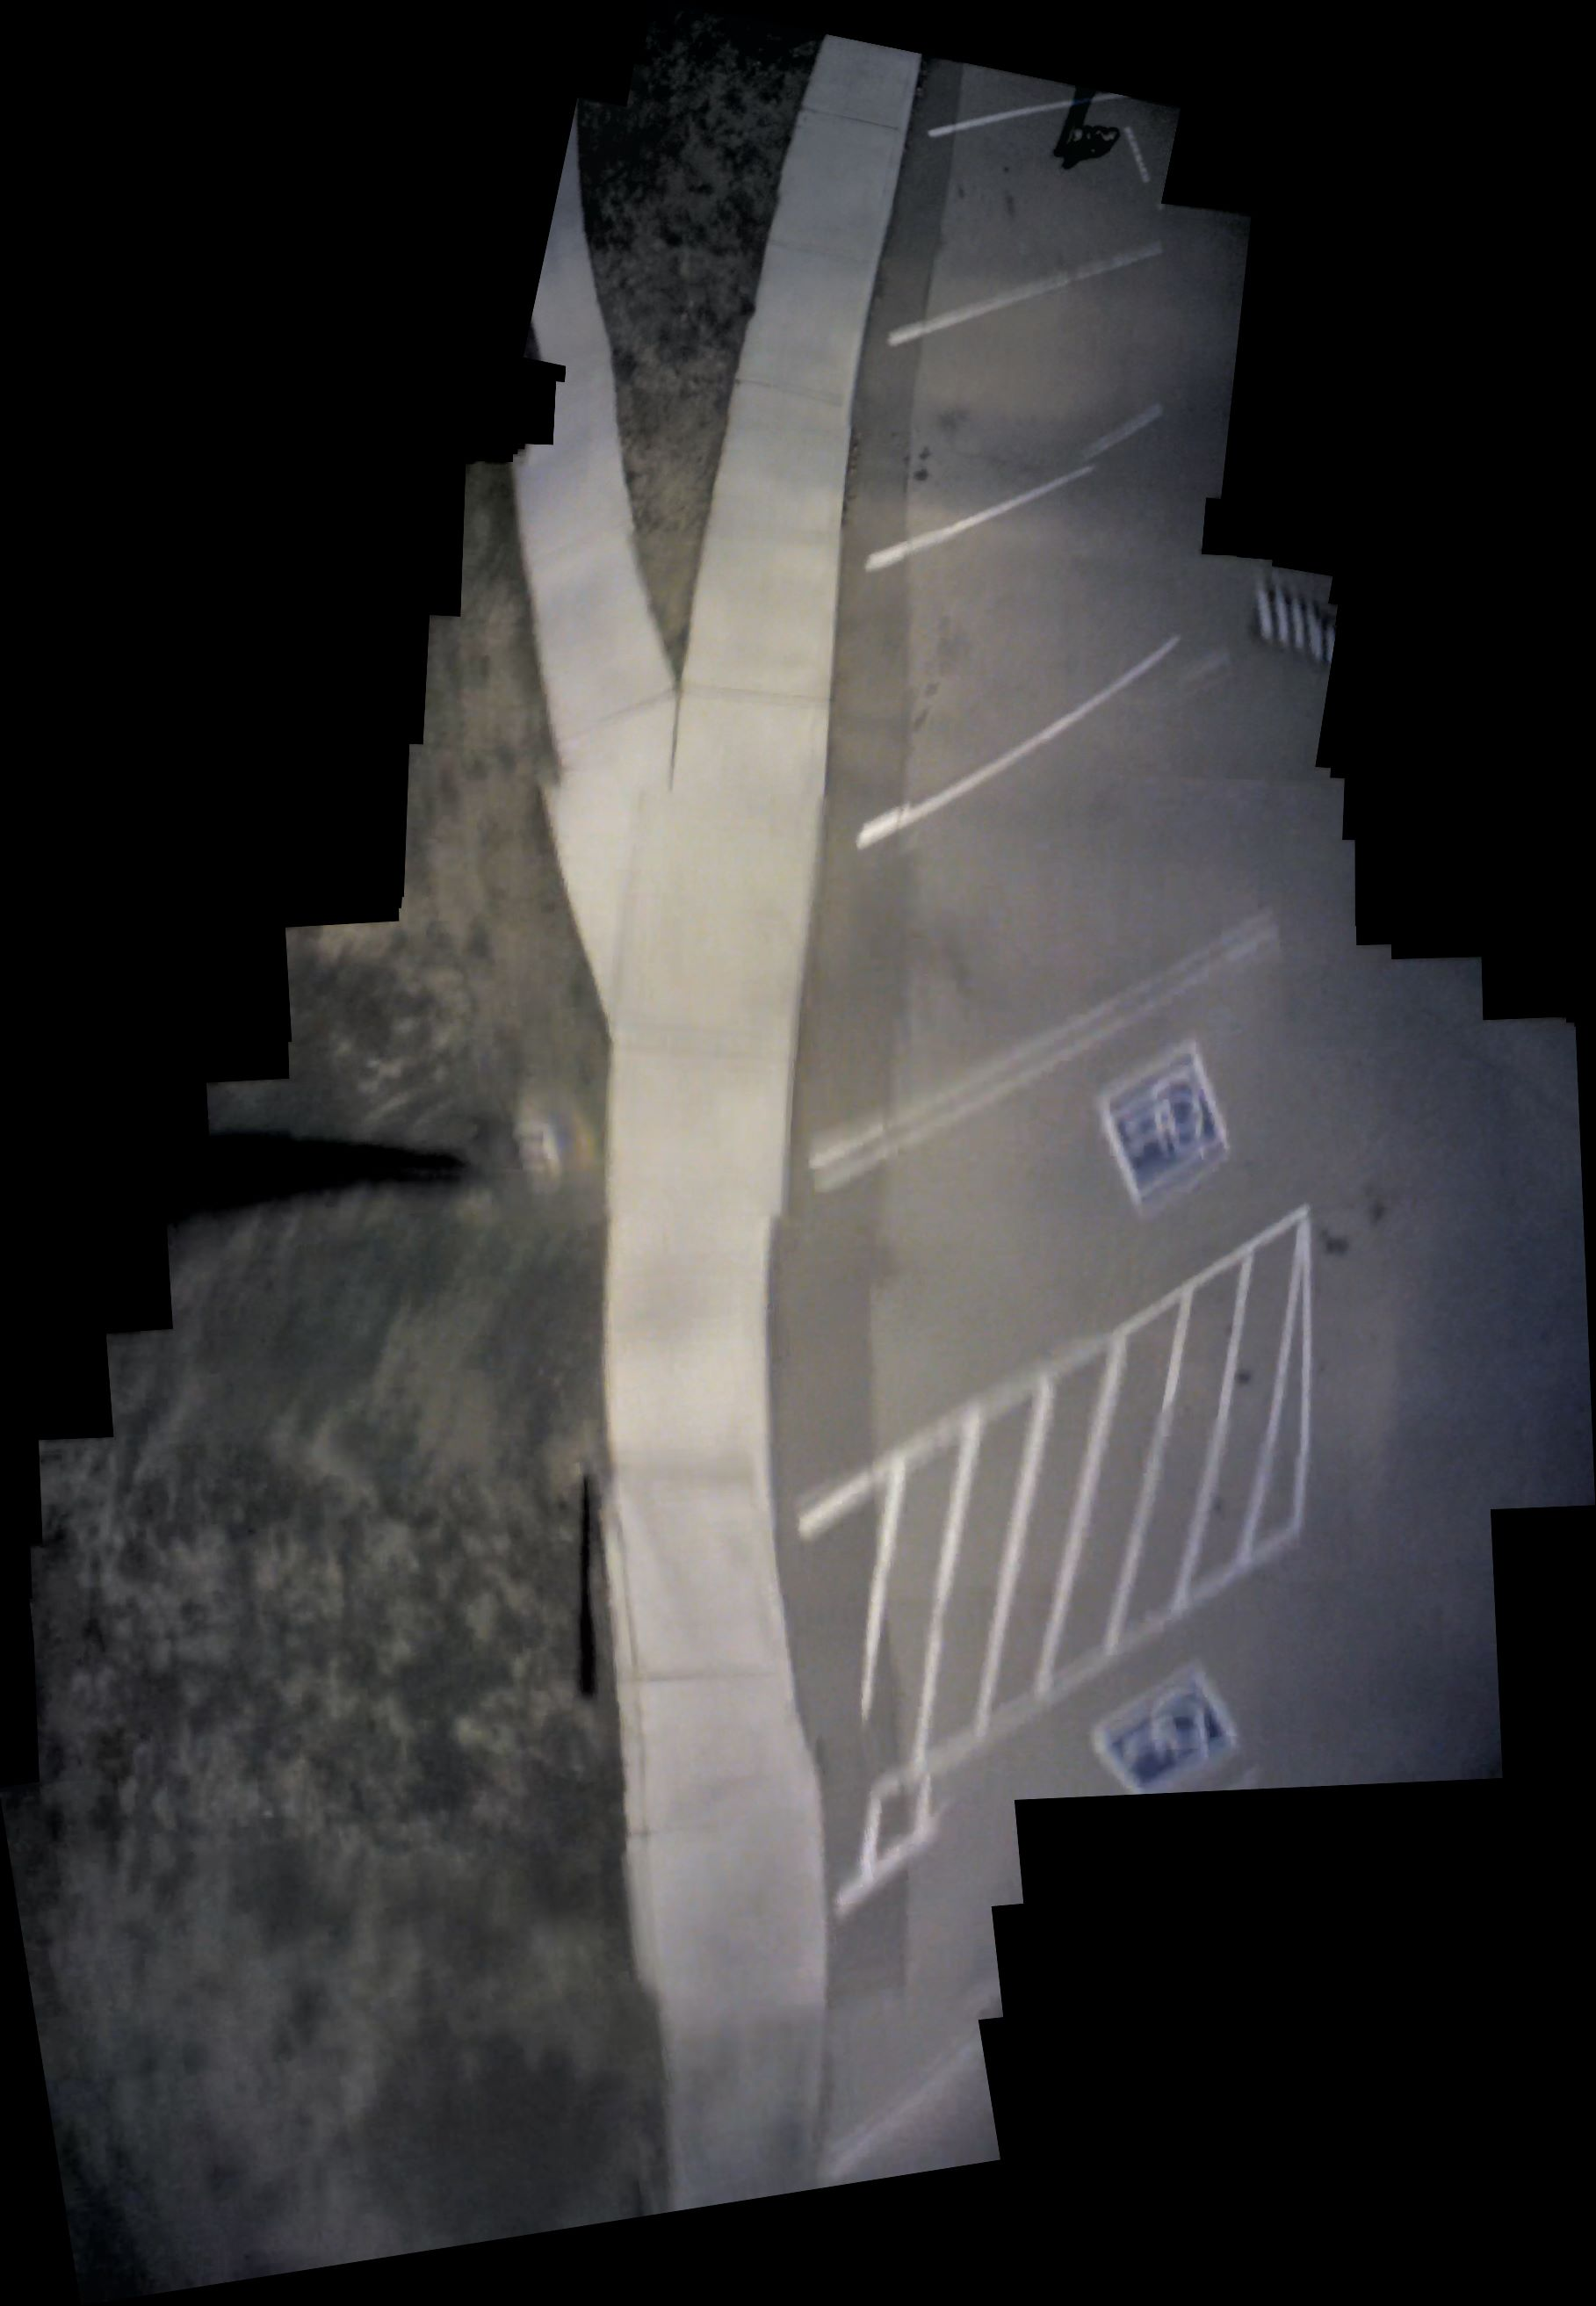
\includegraphics[width=0.95\linewidth]{illustrations/maps/KennedySidewalkStitch}
	\end{minipage}
	\begin{minipage}{.5\textwidth}
		\caption{Comparison of satellite and stitch quality}
		\label{fig:DebrisEarth}
		\centering
			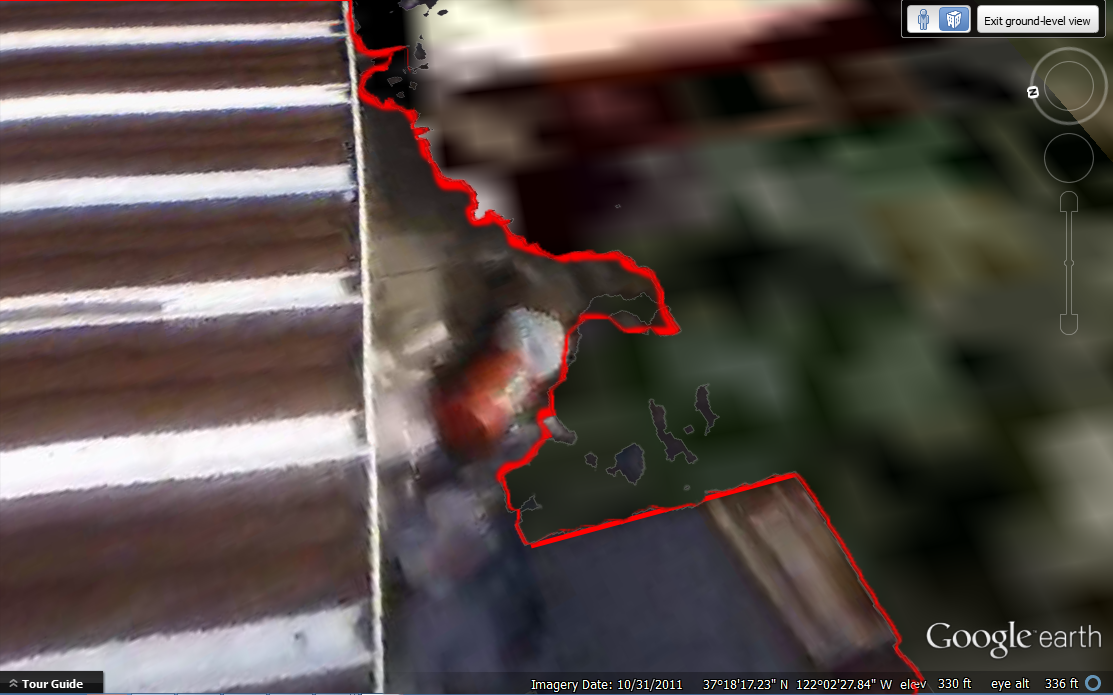
\includegraphics[width=0.95\linewidth]{illustrations/maps/debris}
		\linebreak
		\caption{Stitched image of a playground}
		\label{fig:Playground}
		\centering
			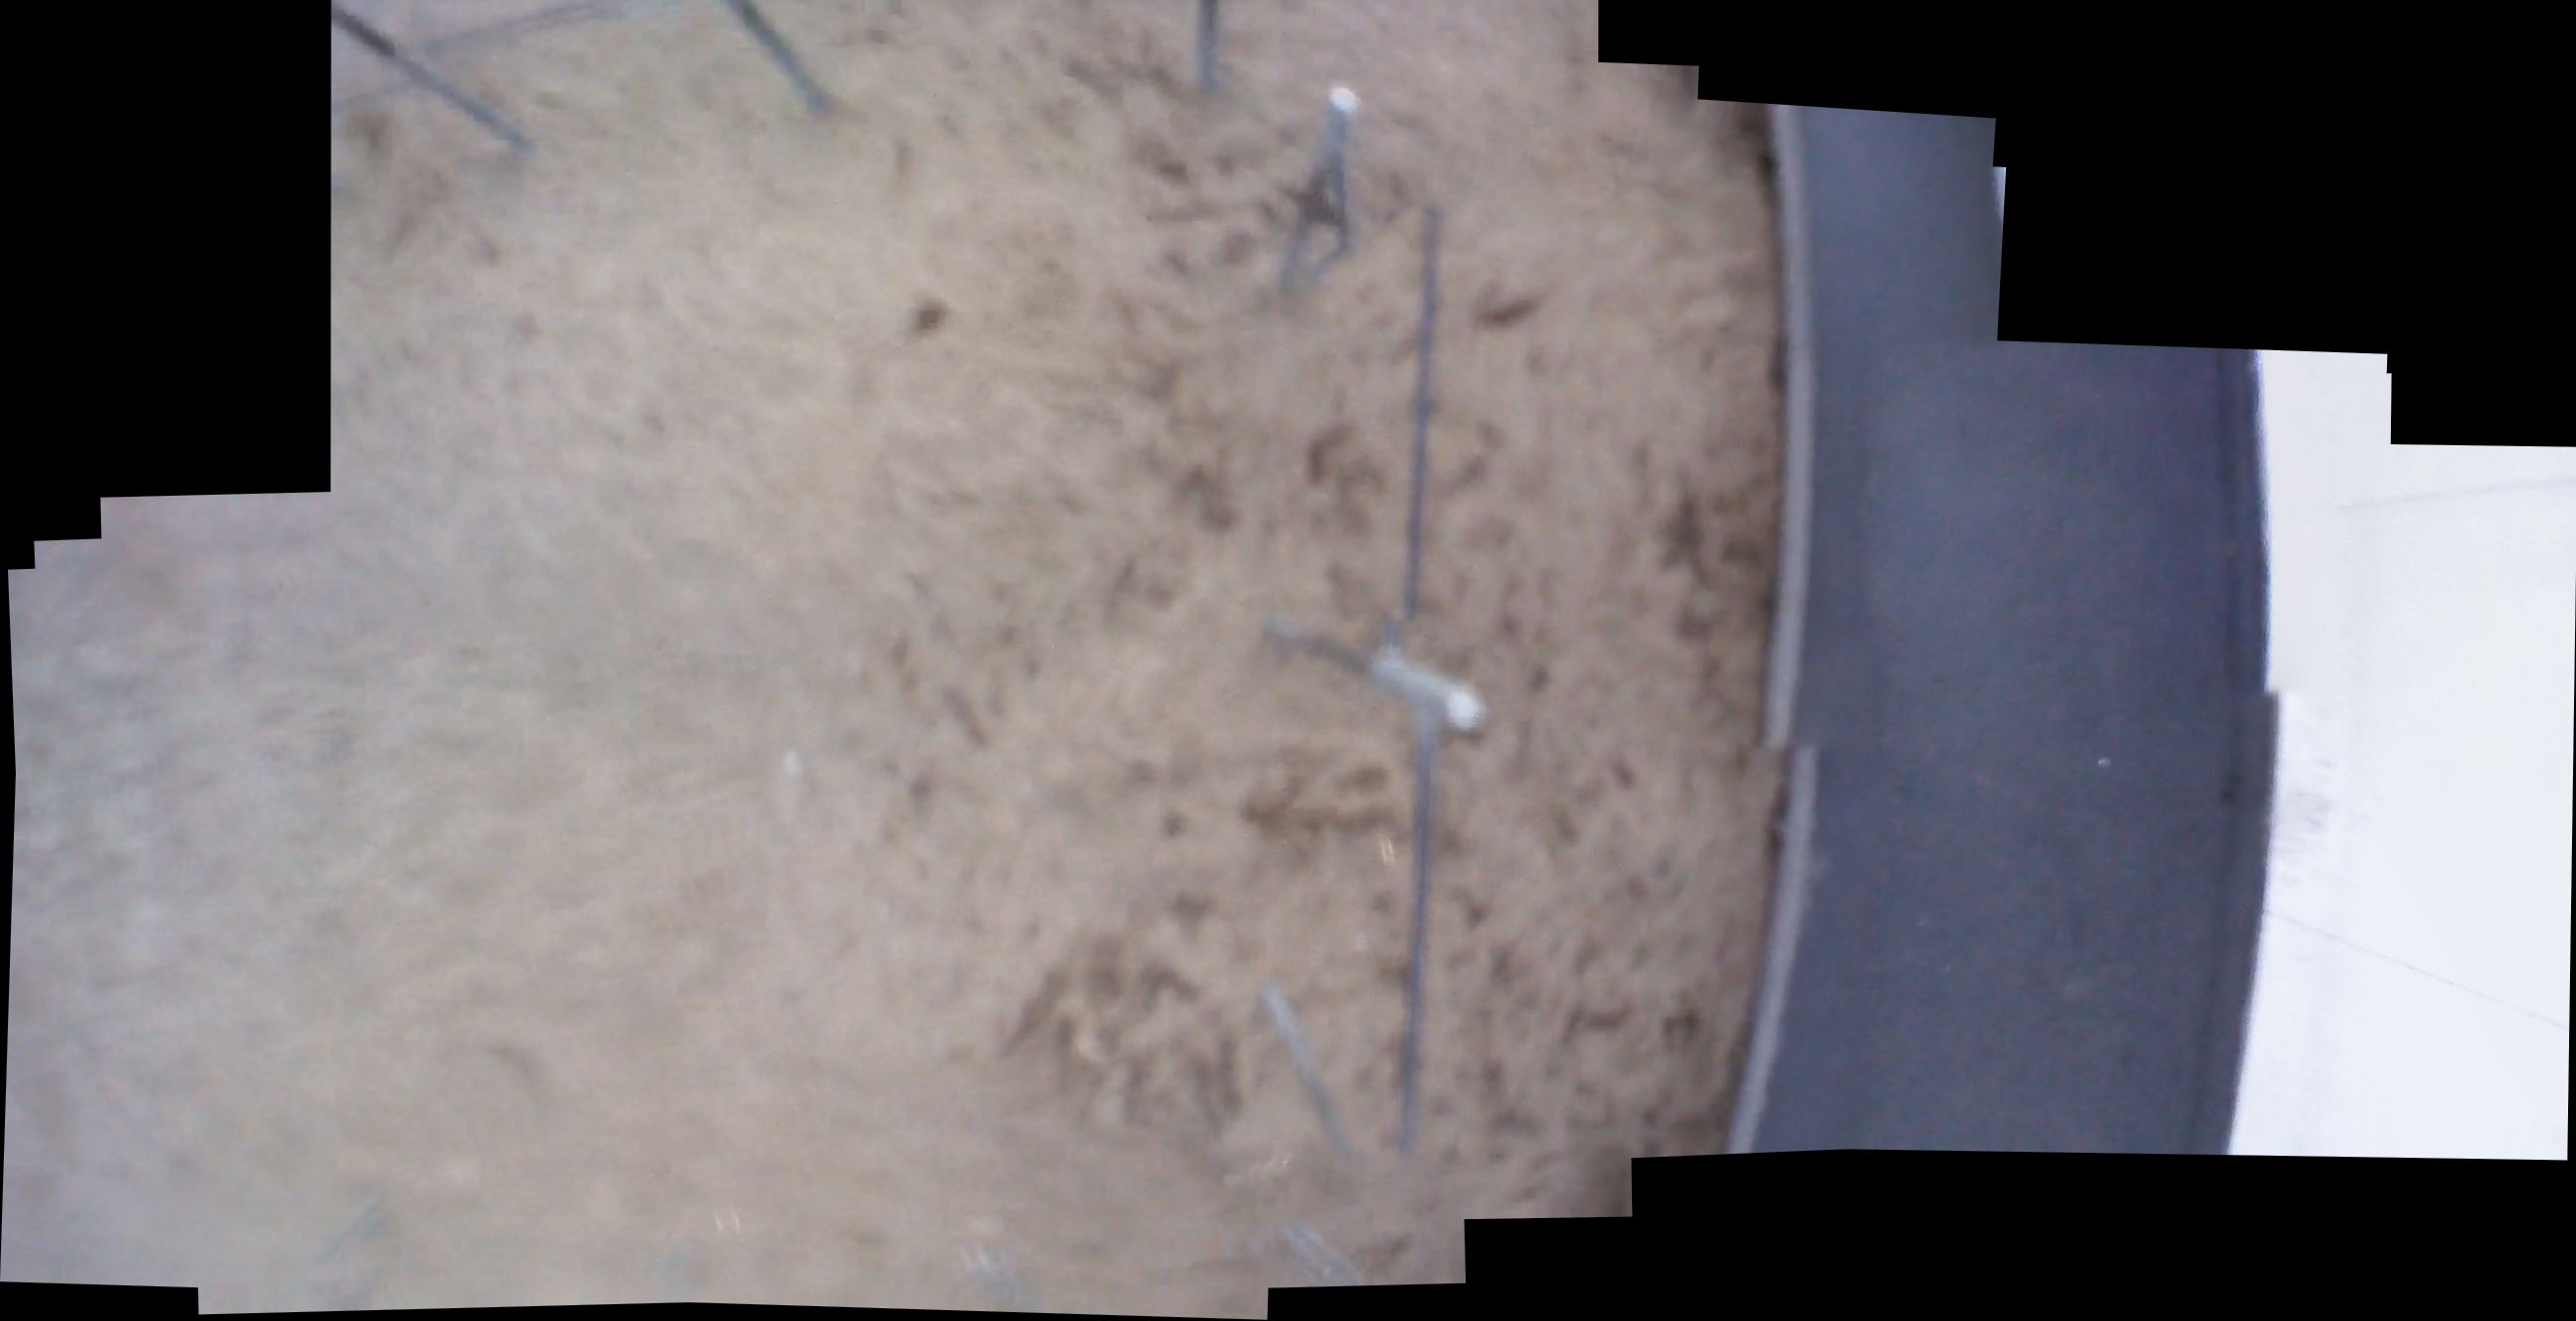
\includegraphics[width=0.95\linewidth]{illustrations/maps/tanbark_structures}
	\end{minipage}
\end{figure}
\clearpage
\begin{figure}[H]
	\caption{Map created from house flyover}
	\label{fig:HouseStitch}
	\centering
		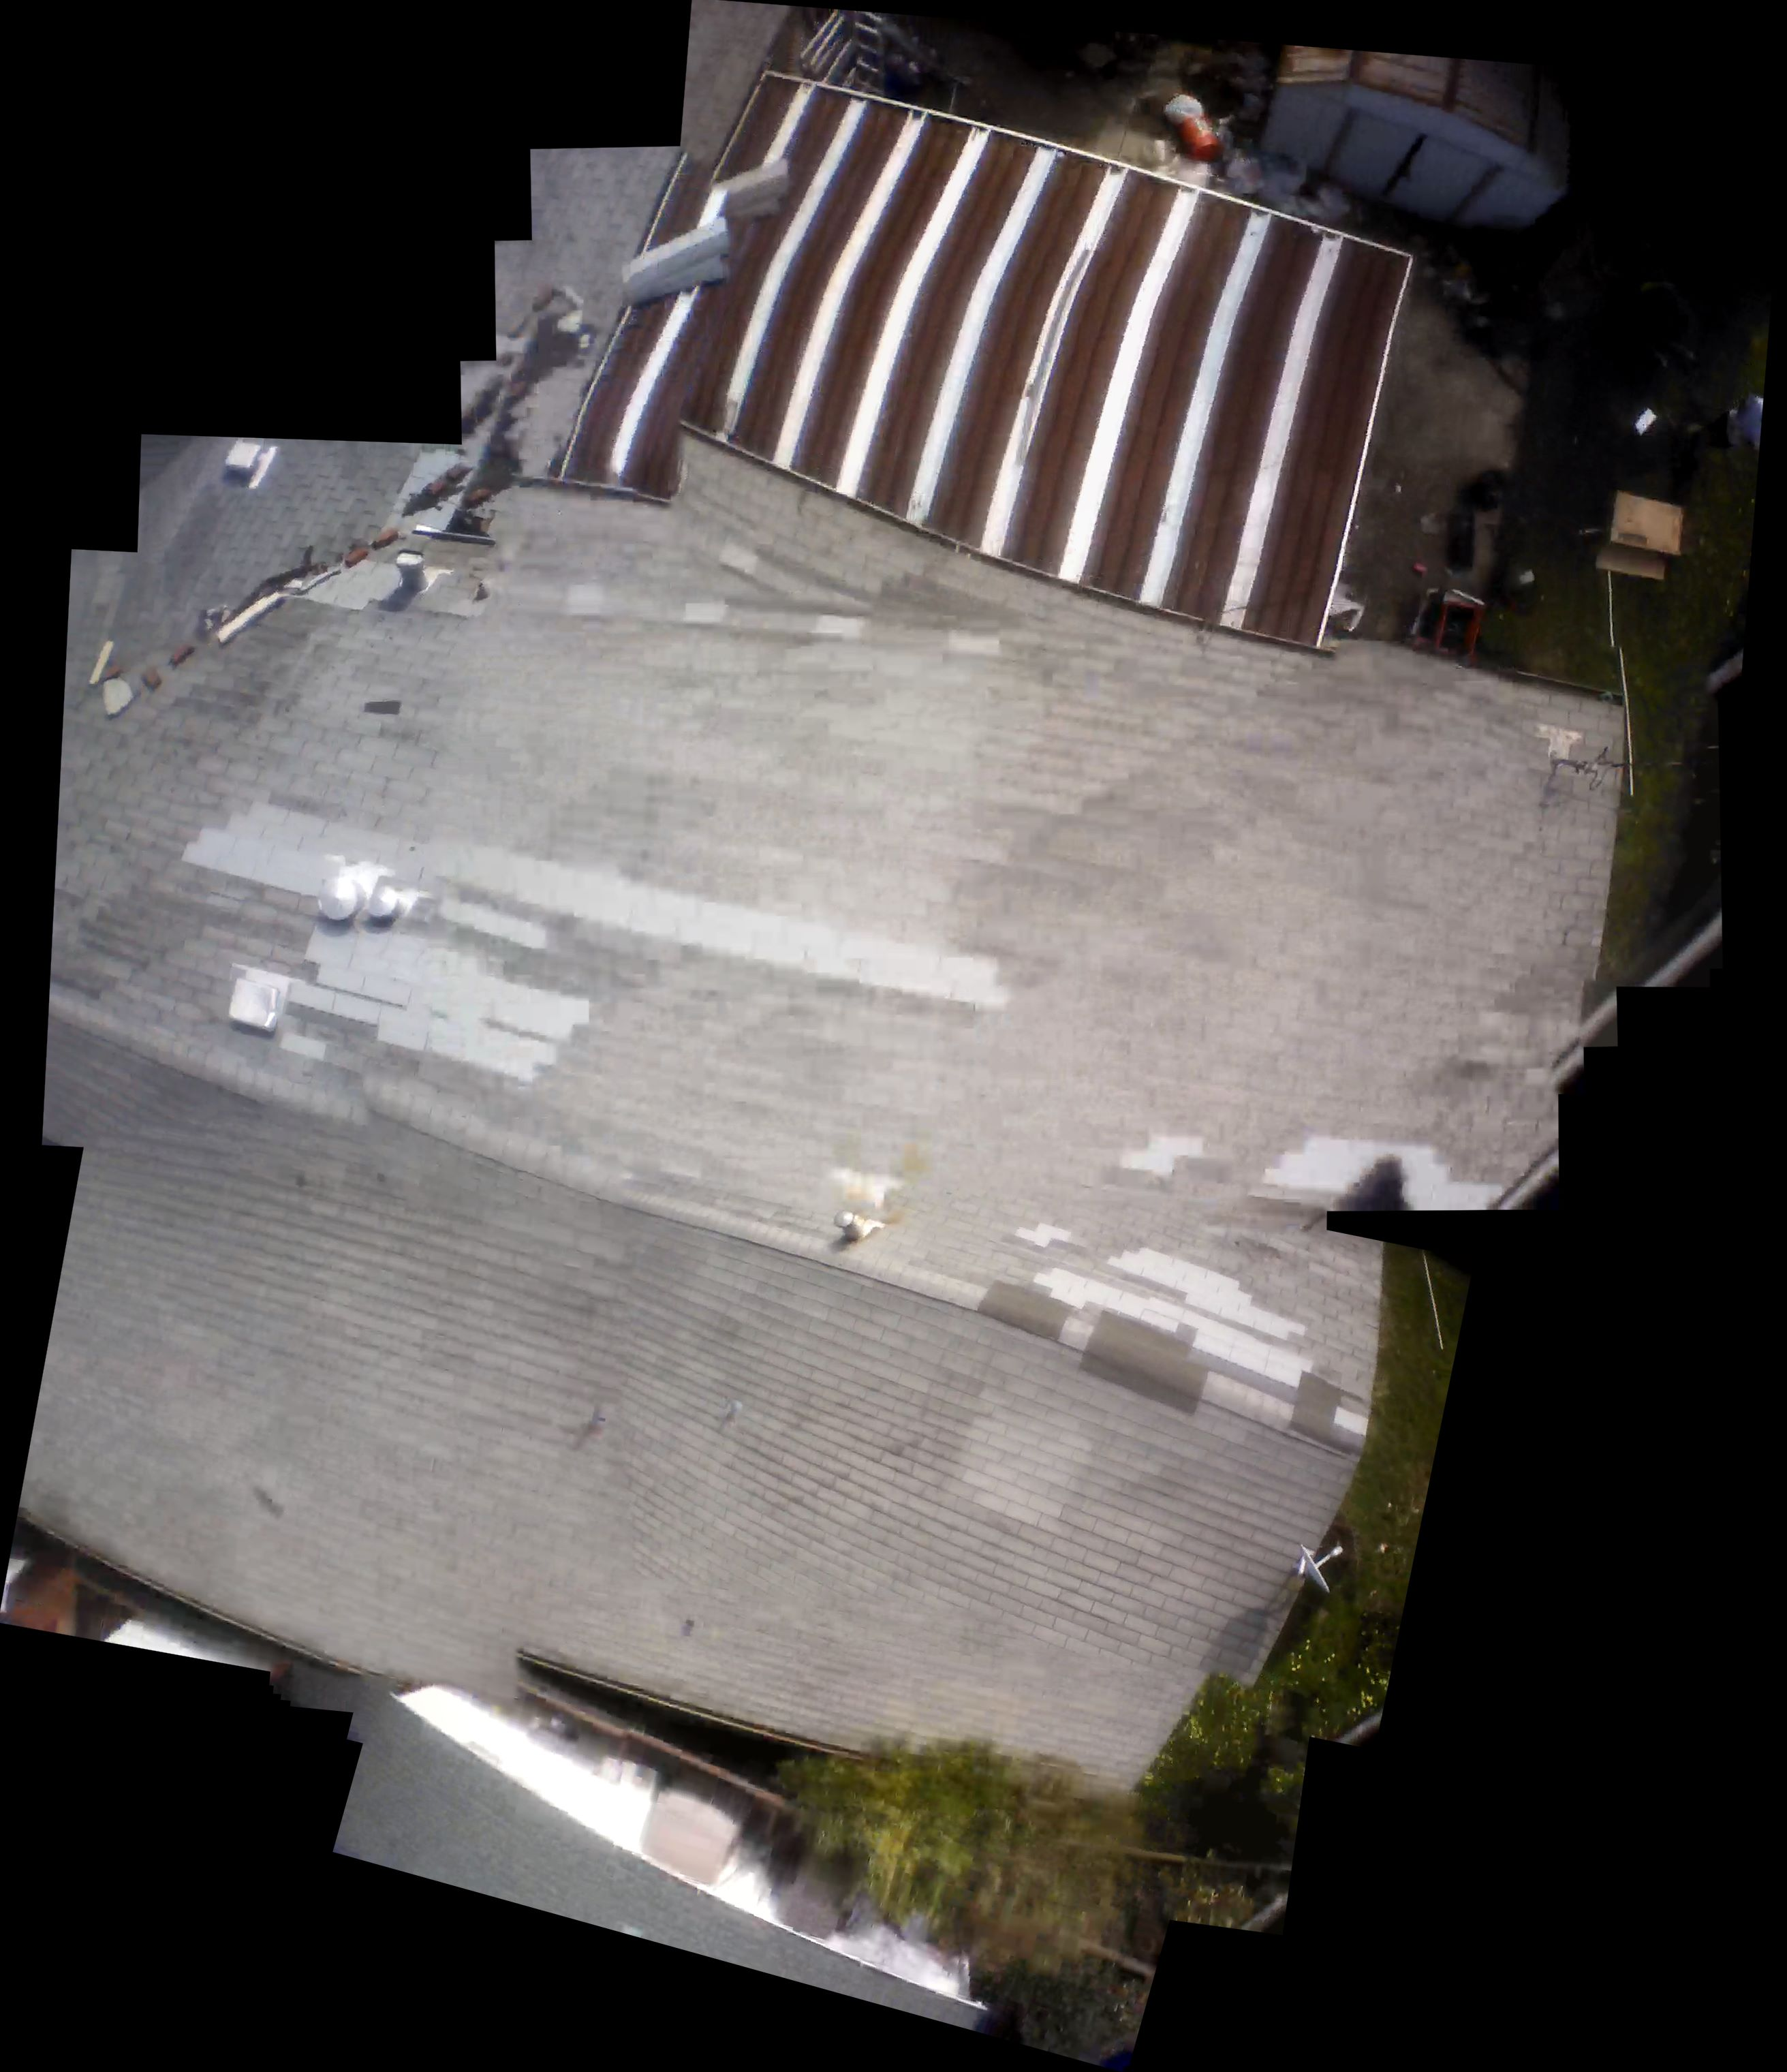
\includegraphics[width=\textwidth]{illustrations/maps/house}
\end{figure}

\begin{figure}[H]
  \caption{Panoramic stitched image from 720 p front camera above rooftops}
  \label{fig:StellingStitch}
  \centering
    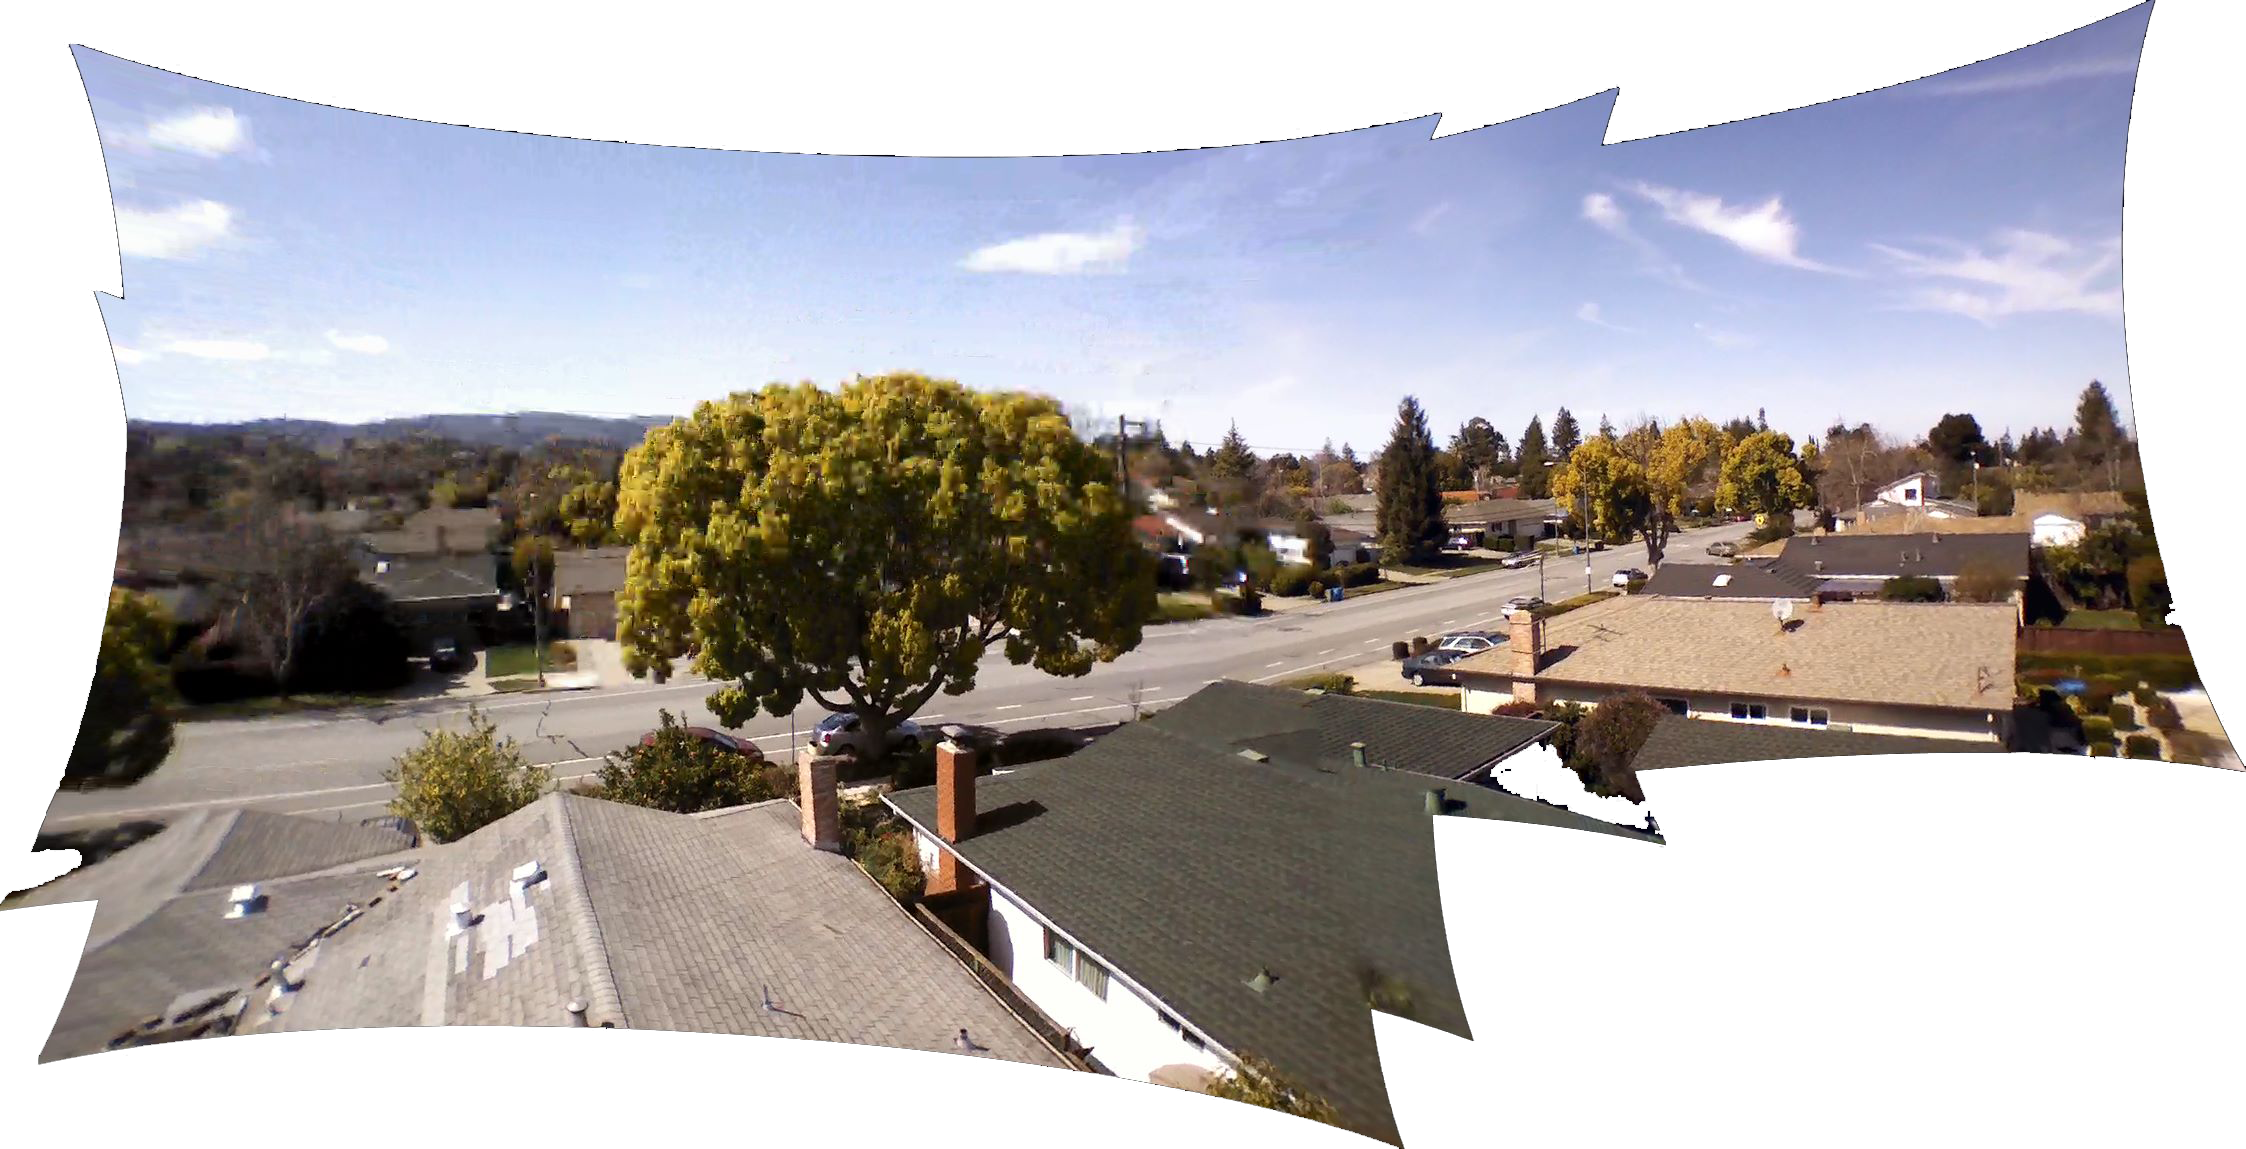
\includegraphics[width=\textwidth]{illustrations/maps/stelling}
\end{figure}


%\begin{figure}[H]
%	\caption{Stitch from low resolution stabilization camera}
%	\label{fig:BackyardStitch}
%	\centering
%		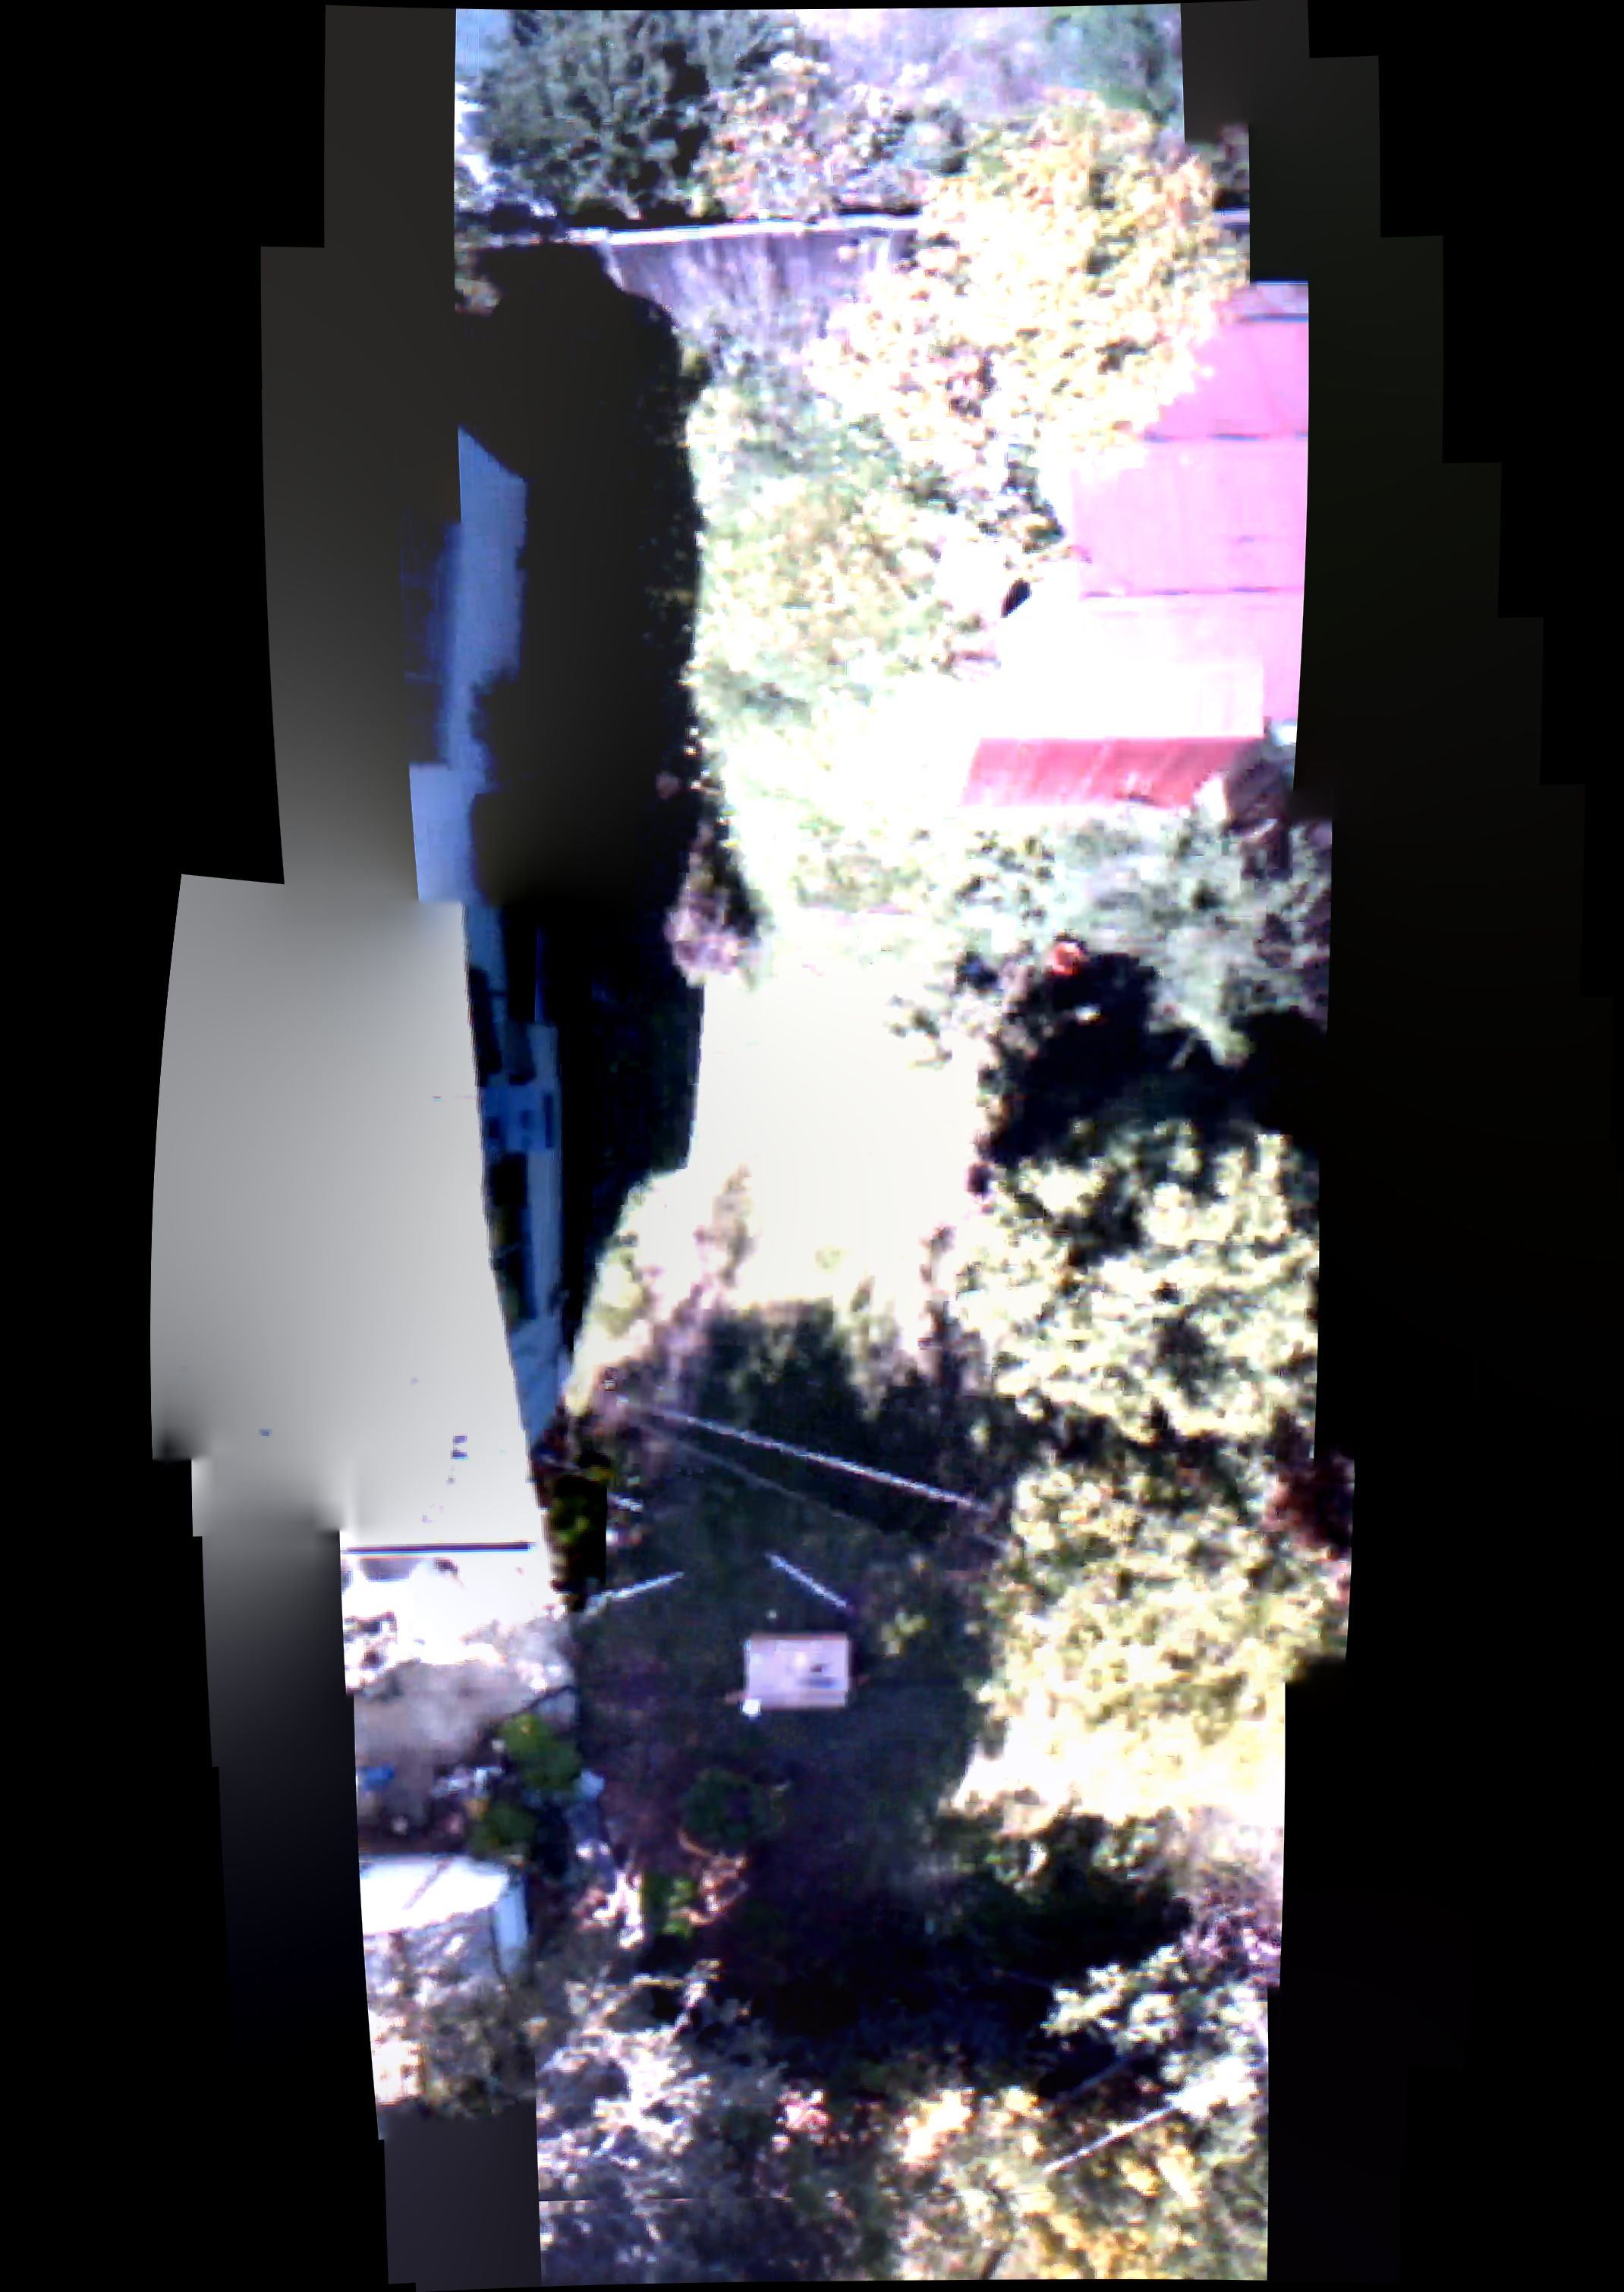
\includegraphics[width=.3\textwidth]{illustrations/maps/backyardOverhead2}
%\end{figure}
% !TEX root = ../paper.tex

\section{Discussion}						% 3-4 pages
											% major lessons

\subsection{Design Criteria Analysis}

Our final prototype met all of our initial design criteria, satisfying the engineering goal.

\begin{enumerate}
	\item The UAV can withstand wind speeds up to 15 km/h without significant degradation in flight ability. Drifting does occur, however, and higher wind speeds may result in a drone becoming unpredictable. Winds past 30 km/h could result in the drone bailing due to inversion. However, given enough altitude, the drone can recover from free-fall.
	\item A GPS unit, barometer, ultrasonic distance sensor and an accelerometer were used.
	\item $\$500$ total net cost for a single unit
	\item We included a 720p front camera for generating panoramas, 5 megapixel bottom facing phone camera for mapping, 240p stabilization camera. In panoramas, objects as small as $5$ cm can be resolved - this is an \textbf{order of magnitude better than satellite imagery} and allows for victim detection.
%	\item Arduinos can interface with the drone to send additional data to the server if needed. However, we ruined a drone when a crash resulted in a short that destroyed one quadcopter.
\end{enumerate}

\subsection{Impact and Applications}

\subsubsection{Disaster Response}
Aerial maps allow for fast damage assessment. Imagery is automatically analyzed for faces and keypoints, then stitched and superimposed onto maps. Load is taken off emergency and recovery workers, allowing their efforts to be focused on investigating the detected interest areas. Up to date maps of fire, flood, earthquake and hurricane damaged areas are created where the delay from satellites is intolerable.

\subsubsection{Search and Rescue}
Since the PC server handles drone flight, operators only need to select a search area. This allows rapid situation assessment without having to wait for trained aircraft or helicopter pilots to arrive. Fast response is critical in search and rescue operations where survival chances decline very quickly

\subsubsection{Indoor Mapping}
Search and rescue teams can 3-dimensionally map the interior of damaged buildings to locate survivors without self-endangerment. The maneuverability of quadrotors allows navigation through doors, windows and skylights.

\subsection{Comparison to Alternate Solutions}

\begin{description}
	\item[SATELLITES:] The final system produces images with up to 10 times higher angular resolution than the best available satellite imagery. A network of our UAVs can be deployed over a city immediately after a disaster, whereas imagery from satellites would not be available for several days.
	\item[PILOTED AIRCRAFT:] A full scale helicopter can cover much more ground than an individual quadcopter, but must fly at a high altitude, limiting the resolution of imagery. The coverage limitation was addressed by developing a network of multiple drones that map a city in pieces and progressively enhance the resolution of devastated areas. Additionally, none of the alternate solutions address the problem of indoor mapping.
	\item[OTHER UAVs:] Each of our quadrotor systems is under $\$500$, far more inexpensive than existing UAVs that have been used for search and rescue. Many alternate UAVs are piloted and simply return a video feed. This requires at least one operator per drone, when manpower should be focused on rescue.
\end{description}
% !TEX root = ../paper.tex

\section{Conclusions and Future Work}		% 1-3 pages

\textbf{We effectively produce up to date, high resolution maps and models that assist with fast damage
assessment in disaster response, search and rescue, and indoor survivor search. Our system has an order of
magnitude better angular resolution than current satellite imaging, and each drone is under \$500,
compared to current UAVs ranging from tens to hundreds of thousands of dollars.}

\subsection{How we met our Project Goals}

After developing 3 main hardware prototypes, our final drone uses a self contained image and telemetry
collection unit, while initially we used the Arduino microprocessor.
Our system 1) captures low resolution imagery with a high altitude drone to 2) automatically identify damaged areas where 3) low altitude drones capture very high resolution imagery. Data is 4) presented on existing aerial mapping tools used by first responders.

Within dangerous buildings, quadrotors with 3D cameras capture full 3D maps of building interiors. Bodies are detected and the models are sent to doctors for remote diagnosis.
This technology saves the lives of first responders as they do not need to search inside collapsing buildings.

\subsection{Further Research}
In the future, we will investigate alternate UAV technologies to allow for more carry-weight. In turn, we could mount higher quality imaging equipment and additional sensors. After looking into other rotor based systems, we would develop an imaging platform based on a fixed-wing UAV. Fixed wing planes can cover large areas in one flight, although we would not be able to use the same system to map the interiors of buildings.

As we develop the project, we may develop an networking solution between drones without a centralized PC server. Tasks and computation would be divided between drones with peer to peer communication. This would allow for massive scale deployments of drones across a city.

\clearpage

% \section{References}						% Any length
% \input{./sections/References.tex}

\section{References}

	\subsection{References}
	\singlespacing\bibliography{bibliography}
	
%	\subsection{Background}
	\singlespacing\nocite{*}
%	\nocite{NeuroForge:OpenCV}
	
	% [1] (Figure 1) - $http://www.ted.com/talks/vijay_kumar_robots_that_fly_and_cooperate.html$
	
	
	%% TO READ
	% http://ntrs.nasa.gov/archive/nasa/casi.ntrs.nasa.gov/20090036330_2009036511.pdf (2009) - UAVs for tornado stuff

\end{document}
